\documentclass[11pt,a4paper]{article}

\usepackage[utf8]{inputenc}
\usepackage[T1]{fontenc}
\usepackage[margin=0.95in]{geometry}
\usepackage{graphicx}
\usepackage{amsmath,amssymb,bm}
\usepackage{array,booktabs,multirow}
\usepackage{setspace}
\usepackage[colorlinks=true,linkcolor=blue!65!black,citecolor=blue!65!black,urlcolor=blue!65!black]{hyperref}
\usepackage{xcolor}
\usepackage{cite}
\usepackage{caption}
\usepackage{enumitem}
\usepackage{float}

\graphicspath{{./}{./assets/}{./Review3_PHASE1/assets/}}

\setstretch{1.14}
\setlength{\parskip}{0.45em}
\setlength{\parindent}{0pt}

\begin{document}

% ============================================================================
% TITLE BLOCK
% ============================================================================
\begin{center}
    {\large \textbf{Shiv Nadar University Chennai}}\\[2pt]
    {\small Department of Computer Science and Engineering --- Capstone Project Architecture \& Literature Report}\\[10pt]
    \rule{\textwidth}{1.2pt}\\[8pt]
    {\LARGE \textbf{Architectural Evolution of Our UAV Tiny-Object Detector:}}\\[4pt]
    {\large \textbf{Literature Groundwork, Methodological Progression Across Reviews, and System Design}}\\[8pt]
    \textbf{Anjana K} (23011101022) \quad --- \quad \textbf{Lalith Adithyan S} (23011101071) \quad --- \quad \textbf{Guide:} Dr.\ Chandrakala S\\[6pt]
    \rule{\textwidth}{0.8pt}
\end{center}

\vspace{0.3em}

% ============================================================================
% SECTION 1: THE PROBLEM & DATASET CHALLENGES
% ============================================================================
\section{Why Detecting Tiny Objects from Drones Is So Difficult}

Detecting objects from Unmanned Aerial Vehicles (UAVs)---evaluated on standard aerial benchmarks such as \textbf{VisDrone2019-DET}~\cite{du2019visdrone,zhu2021visdrone} and \textbf{DOTA}~\cite{xia2018dota,ding2021dota}---is fundamentally different from standard ground-level object detection on datasets like MS-COCO~\cite{lin2017fpn,lin2017focal}. When a camera is held at eye level or mounted on a car, people and vehicles fill a large portion of the frame and show clear visual details. When a drone flies at 50 to 150 meters altitude, the detector faces four severe real-world obstacles at once:

\begin{enumerate}[leftmargin=1.8em]
    \item \textbf{Extremely Tiny Object Sizes ($< 12\times 12$ Pixels):} As shown in Figure~\ref{fig:dataset_stats}(a), more than \textbf{60.5\%} of the annotated objects in VisDrone2019 (distant pedestrians, cyclists, motorcycles, and cars) are small targets~\cite{wang2021nwd,xu2021dotd}. After a neural network downsamples the image by a factor of 8 (the standard $P_3$ feature map), a $12\times 12$ pixel car shrinks to just $1.5\times 1.5$ grid cells. A single standard pooling or strided layer can wipe out a distant $2\times 2$ pixel motorcycle completely.
    \item \textbf{Overwhelming Background Clutter ($> 98\%$ of the Frame):} All foreground objects combined occupy less than $2\%$ of the image pixels. The remaining $98\%$ is complex urban background---asphalt road markings, building windows, rooftop units, and trees. Standard filters struggle to tell a $6\times 6$ pixel car apart from a $6\times 6$ patch of road texture.
    \item \textbf{Shadows, Night Lighting, and Camouflage:} Drones capture scenes under harsh sunlight, night-time street lighting, and deep building or tree shadows~\cite{shang2026badanet,sun2020drone}, as shown in Figure~\ref{fig:dataset_gt}. A dark sedan parked on dark asphalt in the shade has almost zero brightness contrast against the road in standard RGB channels, causing normal edge detectors to miss its boundary.
    \item \textbf{Tightly Packed Crowds and Heavy Occlusion:} As shown in Figure~\ref{fig:dataset_stats}(b), across almost every category in VisDrone2019, $40\%$ to $60\%$ of instances suffer from partial or heavy occlusion~\cite{liang2022fidt,yang2019clusdet}. At traffic signals and plazas, dozens of cars and pedestrians stand bumper-to-bumper. If the network blurs neighboring features together, two touching vehicles get merged into a single box, hurting detection recall.
\end{enumerate}

\begin{figure}[H]
    \centering
    \begin{minipage}{0.47\textwidth}
        \centering
        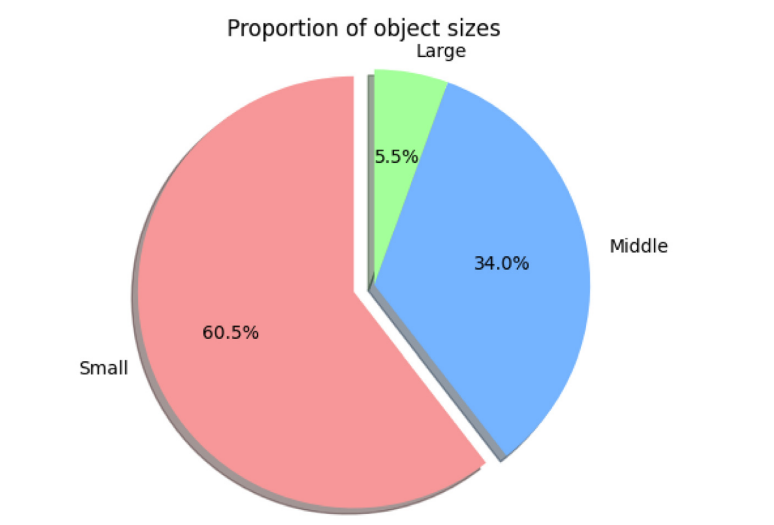
\includegraphics[width=\textwidth]{ObjectSizes.png}
        \par\vspace{2pt}{\small \textbf{(a)} 60.5\% of aerial targets are small ($< 32\text{ px}$).}
    \end{minipage}\hfill
    \begin{minipage}{0.51\textwidth}
        \centering
        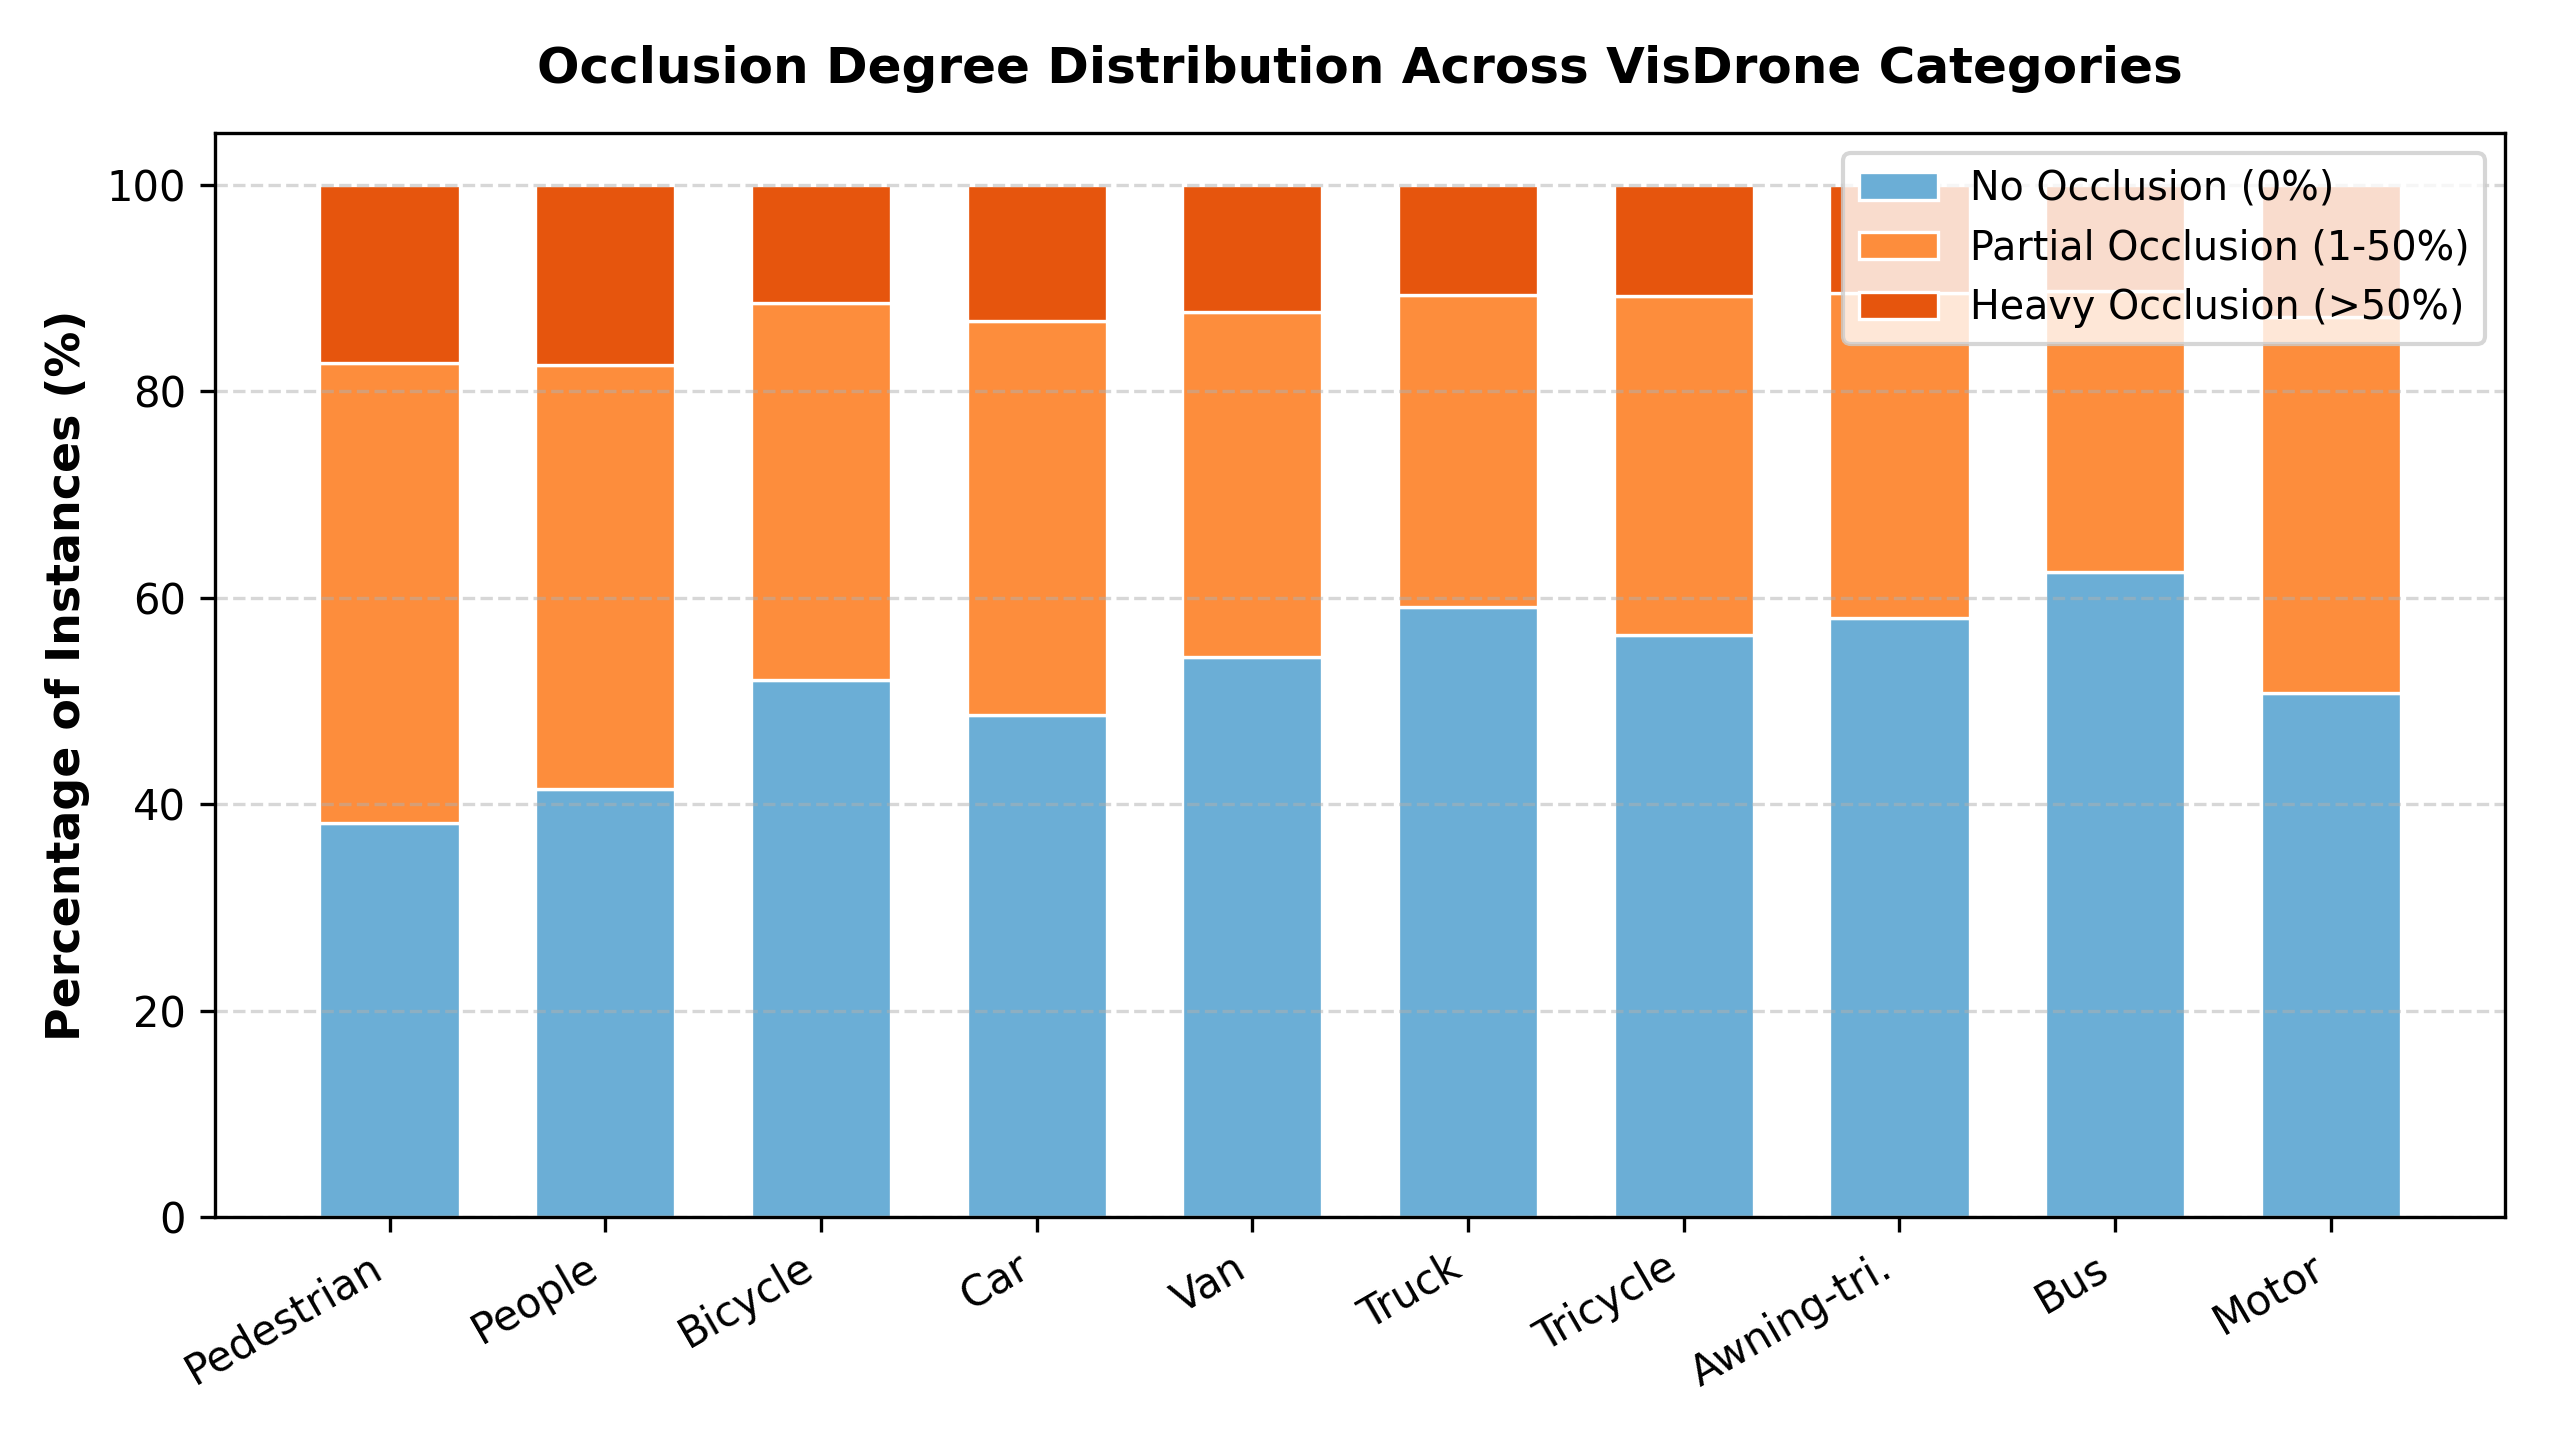
\includegraphics[width=\textwidth]{occlusion_chart.png}
        \par\vspace{2pt}{\small \textbf{(b)} Severe partial and heavy occlusion across all 10 classes.}
    \end{minipage}
    \caption{Key statistical challenges of the VisDrone2019 benchmark: extreme dominance of tiny objects and heavy inter-object occlusion in crowded urban scenes.}
    \label{fig:dataset_stats}
\end{figure}

\begin{figure}[H]
    \centering
    \begin{minipage}{0.48\textwidth}
        \centering
        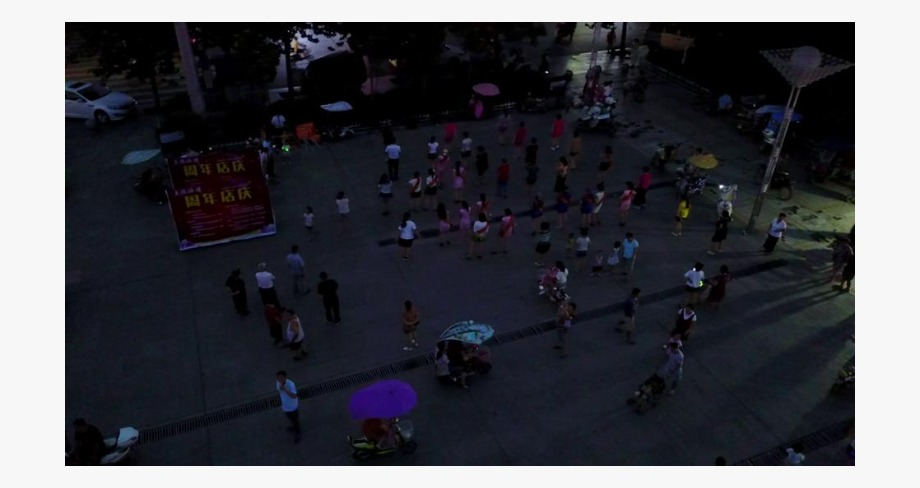
\includegraphics[width=\textwidth]{GT_VisDrone.jpeg}
        \par\vspace{2pt}{\small \textbf{(a)} Raw low-light drone capture.}
    \end{minipage}\hfill
    \begin{minipage}{0.48\textwidth}
        \centering
        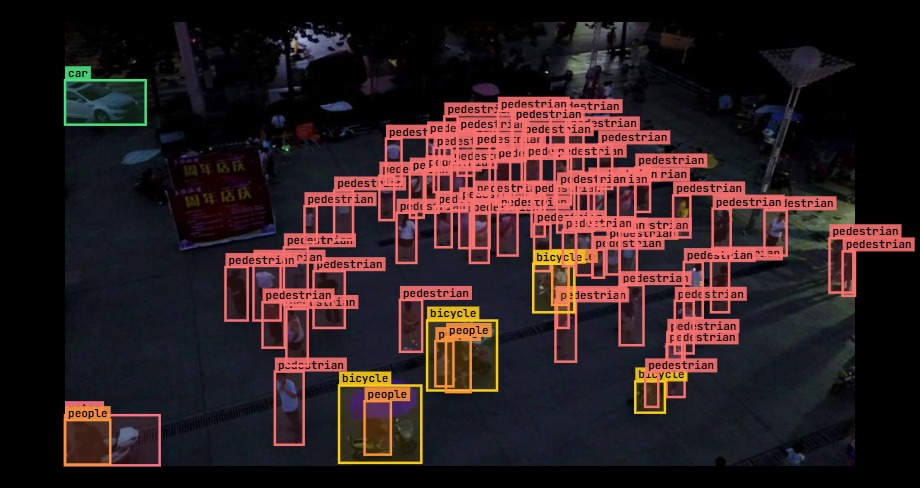
\includegraphics[width=\textwidth]{GT_annotated.jpeg}
        \par\vspace{2pt}{\small \textbf{(b)} Ground-Truth (GT) bounding boxes in a dense crowd.}
    \end{minipage}
    \caption{Visual example from VisDrone2019 showing how low illumination (shadows/night) and dense crowd packing make tiny-object detection exceptionally challenging.}
    \label{fig:dataset_gt}
\end{figure}

\subsection{Dataset Selection: How We Chose VisDrone2019-DET and DOTA as Our Primary Benchmarks}

Before writing any code, one of our most important early decisions in \textbf{Review 0 / Review 1} was choosing the right datasets to train and benchmark our detector. We surveyed existing computer vision datasets across three categories and narrowed down to \textbf{VisDrone2019-DET}~\cite{du2019visdrone,zhu2021visdrone} as our primary drone benchmark and \textbf{DOTA}~\cite{xia2018dota,ding2021dota} as our secondary high-altitude remote-sensing benchmark:

\begin{enumerate}[leftmargin=1.6em]
    \item \textbf{Why Standard Ground-Level Datasets (MS-COCO, Pascal VOC, BDD100K) Were Eliminated:}
    General object detection benchmarks like \textbf{MS-COCO}~\cite{lin2017fpn} capture scenes from eye-level cameras where objects occupy $10\%$ to $60\%$ of the frame and appear upright from the side. A detector trained or evaluated on COCO does not experience top-down camera angles, extreme altitude scaling, or $98\%$ asphalt/rooftop background clutter.
    
    \item \textbf{Why Older / Narrow Aerial Datasets (UAVDT, Stanford Campus, CARPK, DroneVehicle) Were Not Enough Alone:}
    We also evaluated specialized drone datasets: \textbf{CARPK} only contains top-down parking-lot cars (1 class); \textbf{UAVDT} focuses mainly on highway traffic (3 vehicle classes: car, truck, bus) with lower scene diversity; \textbf{Stanford Drone Dataset (SDD)} is recorded from a fixed campus hover mostly for trajectory tracking; and \textbf{DroneVehicle}~\cite{sun2020drone} is specialized for paired RGB--Infrared vehicle detection. While useful for reference, none of them test fine-grained 10-class urban detection across pedestrians, cyclists, tricycles, motorcycles, and heavy traffic simultaneously.

    \item \textbf{Why We Chose VisDrone2019-DET~\cite{du2019visdrone,zhu2021visdrone} as Our Primary Dataset:}
    Collected by the AISKYEYE team at Tianjin University across \textbf{14 different cities} under diverse weather and lighting conditions (bright daylight, overcast, deep building shadows, and night-time street lights), \textbf{VisDrone2019-DET} contains \textbf{10,209 high-resolution drone images} ($6,471$ train, $548$ validation, $1,610$ test-dev) with over \textbf{342,000 manually annotated bounding boxes} across \textbf{10 real-world urban categories} (\texttt{pedestrian}, \texttt{people}, \texttt{bicycle}, \texttt{car}, \texttt{van}, \texttt{truck}, \texttt{tricycle}, \texttt{awning-tricycle}, \texttt{bus}, and \texttt{motor}). We selected it as our primary dataset for three reasons:
    \begin{itemize}[leftmargin=1.2em]
        \item \emph{True Tiny-Object Stress Test:} Over $60.5\%$ of all instances are small ($<32\times 32\text{ px}$), with thousands of targets measuring just $4\times 4$ to $12\times 12$ pixels.
        \item \emph{Extreme Crowds \& Occlusion:} Up to $100+$ objects appear in a single intersection frame, with $40\%$--$60\%$ partial or heavy occlusion (Figure~\ref{fig:dataset_stats}).
        \item \emph{Universal Benchmark Standard:} Every modern aerial detector---including our baseline \textbf{UAVDet}~\cite{yang2026uavdet}, \textbf{UAV-DETR}~\cite{zhang2025uavdetr}, \textbf{Drone-YOLO}~\cite{zhang2023droneyolo}, and \textbf{LUD-YOLO}~\cite{li2026ludyolo}---uses VisDrone2019-DET as its primary leaderboard.
    \end{itemize}

    \item \textbf{Why We Chose DOTA (Dataset for Object deTection in Aerial Images)~\cite{xia2018dota,ding2021dota} as Our Complementary Benchmark:}
    While VisDrone captures low-to-medium altitude oblique and nadir drone views ($50\text{--}150\text{ m}$), \textbf{DOTA}~\cite{xia2018dota,ding2021dota} contains $2,806$ large-scale overhead aerial and satellite images ($800\times 800$ up to $4000\times 4000$ pixels, sliced into $640\times 640$ / $1024\times 1024$ patches) with \textbf{188,282 instances} across \textbf{15 categories} (including \texttt{small-vehicle}, \texttt{large-vehicle}, \texttt{plane}, \texttt{ship}, \texttt{bridge}, \texttt{harbor}, and \texttt{storage-tank}). Pairing \textbf{VisDrone2019} (low-altitude urban drone crowds and oblique angles) with \textbf{DOTA} (high-altitude nadir overhead remote sensing and extreme aspect-ratio structures) ensures our physics-guided architecture is validated across the entire spectrum of aerial imaging!
\end{enumerate}

\subsection{Why We Benchmark Strictly at $640\times 640$ Instead of Giant Image Sizes}
Early in our literature review, we noticed that a few recent papers (such as \textbf{VSCD-UAV}~\cite{yang2026vscduav}, \emph{IGARSS 2026}) reported high accuracy by resizing every input image to $1536\times 1536$ pixels and feeding it into a massive 68-million-parameter YOLOv8-X model paired with a frozen CLIP text encoder~\cite{radford2021clip}. However, when we checked their baseline tables, we found that vanilla YOLOv11-X already achieved almost the exact same score ($43.2\%$ vs.\ $43.5\%$) simply because a $1536\times 1536$ image has \textbf{$5.76\times$ more pixels} than a $640\times 640$ image.

On real drone hardware (such as an onboard NVIDIA Jetson Orin processor), running a 68M-parameter model at $1536\times 1536$ runs at less than 2 frames per second (FPS), making real-time flight impossible. Therefore, top aerial detection papers---\textbf{UAVDet}~\cite{yang2026uavdet}, \textbf{UAV-DETR}~\cite{zhang2025uavdetr}, \textbf{LGI-DETR}~\cite{chen2025lgidetr}, \textbf{Drone-YOLO}~\cite{zhang2023droneyolo}, \textbf{LUD-YOLO}~\cite{li2026ludyolo}, and \textbf{SL-YOLO}~\cite{chen2025slyolo}---strictly evaluate at \textbf{$640\times 640$ resolution}. Keeping our input size fixed at $640\times 640$ with a lightweight $\sim 4.9\text{M}$ parameter budget ensures a fair comparison where our \emph{architecture itself} solves the tiny-object problem.

% ============================================================================
% SECTION 2: OVERVIEW OF THE RESEARCH TIMELINE ACROSS REVIEWS
% ============================================================================
\section{Overview of Methodological Progression Across Project Reviews}

Across \textbf{Review 0, Review 1, Review 2, Review 3 (Phase 1), and Phase 2}, our architectural design progressed through a systematic evaluation of existing literature across six technical domains. We began with general aerial detection paradigms, narrowed down to State-Space Models (Mamba), audited 2D selective scanning behavior, analyzed 12 dynamic and deformable convolution operators, investigated classical scale-space priors, and finally adapted physics-informed refinement networks for object detection.

Table~\ref{tab:review_journey} summarizes this chronological progression across reviews, detailing the technical paradigms investigated at each stage, the empirical or mathematical limitations identified for tiny aerial targets, and the resulting design decisions.

\begin{table}[H]
\centering
\caption{Chronological Progression of Literature Groundwork and Design Decisions Across Project Reviews.}
\label{tab:review_journey}
\renewcommand{\arraystretch}{1.12}
\footnotesize
\begin{tabular}{p{2.2cm} p{3.8cm} p{4.6cm} p{3.8cm}}
\toprule
\textbf{Project Stage} & \textbf{Technical Paradigm \& Literature} & \textbf{Identified Limitations on Tiny Aerial Targets} & \textbf{Resulting Architectural Decision} \\ \midrule
\textbf{Stage 1} \newline (\emph{Review 1: Detector Paradigms}) & 
$\bullet$ Patch Cropping (\cite{yang2019clusdet,li2020dmnet,yang2022querydet,yuan2023cfinet,akyon2022sahi}) \newline
$\bullet$ Vision Transformers (\cite{carion2020detr,zhu2020deformabledetr,rao2021dynamicvit,lv2024rtdetr,zhang2025uavdetr,chen2025lgidetr}) \newline
$\bullet$ Aerial YOLOs (\cite{zhang2023droneyolo,zhang2024ffcayolo,wang2024mffci,li2026ludyolo,chen2025slyolo}) &
$\bullet$ Cropping 20 sub-patches slows inference by $5\times$--$10\times$ and loses global road context. \newline
$\bullet$ Quadratic attention ($O(N^2)$) is too heavy on high-res $P_2$ ($160\times 160$) grids (20M--42M params). \newline
$\bullet$ Pure CNNs have limited $3\times 3$ local receptive fields. &
Selected \textbf{CNN--Mamba Hybrids} (\cite{gu2022s4,gu2023mamba,wang2024mambayolo,yang2026uavdet}) to capture global context in linear $O(N)$ time within 4.8M parameters. \\ \midrule

\textbf{Stage 2} \newline (\emph{Review 2: State-Space Models}) &
$\bullet$ Visual SSMs: S4~\cite{gu2022s4}, Mamba~\cite{gu2023mamba}, VMamba~\cite{liu2024vmamba}, Spatial-Mamba~\cite{xiao2024spatialmamba}, MambaIRv2~\cite{guo2025mambairv2}, Mamba-YOLO~\cite{wang2024mambayolo}, UAVDet~\cite{yang2026uavdet}. &
$\bullet$ Code audit of \texttt{UAVDet} showed its backbone had \emph{zero} Mamba blocks. \newline
$\bullet$ Uncalibrated 2D scans carry $>98\%$ background clutter into tiny $6\times 6$ objects (\textbf{memory bleed}). \newline
$\bullet$ No cross-scale Mamba scan existed in the neck ($S_4 \rightarrow P_1$). &
Designed \textbf{Boundary-Gated Mamba} in the backbone to flush background state at edges and \textbf{Scale-Axis Mamba} in the neck. \\ \midrule

\textbf{Stage 3} \newline (\emph{Adaptive \& Deformable Convolutions}) &
$\bullet$ Deformable: DCNv1--v3~\cite{dai2017dcnv1,zhu2019dcnv2,wang2023internimage}, Def.\ Kernels~\cite{gao2020deformablekernels}. \newline
$\bullet$ Dilated: SAC~\cite{qiao2021detectors}, Scale-Adaptive~\cite{zhang2017sac}, FADC~\cite{chen2024fadc}, PKINet-v2~\cite{cai2024pkinet,cai2026pkinetv2}. \newline
$\bullet$ Dynamic: DynConv~\cite{chen2020dynamic}, ODConv~\cite{li2022odconv}, Involution~\cite{li2021involution}, PAC~\cite{su2019pac}, CoordConv~\cite{liu2018coordconv}. &
$\bullet$ \textbf{SAC} uses a $5\times 5$ average pool ($91\%$ background over a 1.5-cell car) and blurs peaks across dilations 1 and 3. \newline
$\bullet$ \textbf{DCNv2} predicts 18 unconstrained offsets that drift off textureless targets into road markings. \newline
$\bullet$ Dynamic/ODConv rely on global pooling ($98\%$ background). &
Demonstrated that unconstrained learned offsets fail on tiny targets; explicit \textbf{mathematical image priors} are required. \\ \midrule

\textbf{Stage 4} \newline (\emph{Scale-Space Priors \& Crowd Losses}) &
$\bullet$ Scale-Space LoG~\cite{lindeberg1994scalespace}, SR-TOD~\cite{cao2024srtod}, Spectral (SFS-Conv~\cite{li2024sfsconv}, SET~\cite{sun2025set}). \newline
$\bullet$ Crowd Maps (FIDT~\cite{liang2022fidt}) \& Gaussian Losses (NWD~\cite{wang2021nwd}, RFLA~\cite{xu2022rfla}, DotD~\cite{xu2021dotd}). &
$\bullet$ Grayscale edges fail in shadows; FFT cutoffs cause Gibbs ringing around crowded cars. \newline
$\bullet$ Gaussian heatmaps merge adjacent cars into one blob; IoU loss drops $35\%$ on a 1-px shift. &
Implemented \textbf{Opponent-Color LoG Priors}, \textbf{FIDT center-peak maps}, and \textbf{GIWD loss} in Phase 1 (V1). \\ \midrule

\textbf{Stage 5} \newline (\emph{Physics-Guided Vision \& Visual Memory}) &
$\bullet$ Physics Networks: PMRNet~\cite{kang2026pmrnet}, Perona--Malik~\cite{perona1990anisotropic}, Weickert~\cite{weickert1999coherence}, ST-OBB~\cite{yang2024stobb}, PGBL~\cite{liao2026pgbl}, BADANet~\cite{shang2026badanet}, DeCoF~\cite{liu2025decof}, SPD-Conv~\cite{sunkara2022spd}. \newline
$\bullet$ Visual Prompting: CLIP~\cite{radford2021clip}, EVP~\cite{liu2023evp}, VCP~\cite{wang2025vcp}, PET-DINO~\cite{fu2026petdino}. &
$\bullet$ Segmentation potential ($U=1-\hat{Y}$) erases object centers needed for box anchors; stride-2 skip deletes $75\%$ of pixels. \newline
$\bullet$ CLIP text encoders (150 MB) add unnecessary overhead for 10 fixed classes. &
Formulated \textbf{Symp-STEConv}, lossless \textbf{RGDS}, and a 0.12 MB \textbf{VCP + PET-DINO Visual Memory Bank} for Phase 2 (V2). \\ \bottomrule
\end{tabular}
\end{table}

% ============================================================================
% SECTION 3: DEEP DIVE INTO OUR EXPLORATORY GROUNDWORK (6 DOMAINS)
% ============================================================================
\section{Detailed Literature Groundwork Across Six Technical Domains}

Before presenting our final system architecture, this section details the prior literature evaluated across six technical domains, the specific mechanisms employed by those methods, and the analytical reasons why each approach was either eliminated or adapted for aerial tiny-object detection.

\subsection{Domain 1: Aerial Detection Paradigms (Patch-Cropping, DETRs, and YOLOs)}

At the outset of Review 1, existing aerial object detectors were categorized into three primary architectural paradigms:

\subsubsection*{1. Two-Stage ``Coarse-to-Fine'' Patch Cropping Pipelines}
Because tiny objects occupy a small fraction of the image, early VisDrone pipelines focused on cropping and magnifying high-density regions:
\begin{itemize}[leftmargin=1.5em]
    \item \textbf{ClusDet}~\cite{yang2019clusdet} (\emph{ICCV 2019}) and \textbf{DMNet}~\cite{li2020dmnet} (\emph{CVPRW 2020}) train a coarse network to predict vehicle and pedestrian cluster regions, crop 15 to 30 sub-patches around those clusters, upsample each patch, and execute a second detection pass on every crop.
    \item \textbf{QueryDet}~\cite{yang2022querydet} (\emph{CVPR 2022}) accelerates this process by applying sparse convolutions only around coarse query locations on high-resolution feature maps, while \textbf{CFINet}~\cite{yuan2023cfinet} (\emph{ICCV 2023}) employs coarse-to-fine proposal imitation learning.
    \item \textbf{SAHI (Slicing Aided Hyper Inference)}~\cite{akyon2022sahi} (\emph{ICIP 2022}) partitions each test image into overlapping windows at inference time and merges predictions via NMS.
    \item \textbf{Technical Limitation:} Executing the detector 16 to 32 times per frame increases inference latency by $5\times$ to $10\times$, precluding real-time onboard UAV deployment. Moreover, isolated sub-patches sever global scene layout (such as roadway boundaries versus building roofs), increasing false-positive detections on background structures.
\end{itemize}

\subsubsection*{2. Vision Transformers and End-to-End DETR Architectures}
We next evaluated whether Transformer self-attention could provide global context for small-target localization:
\begin{itemize}[leftmargin=1.5em]
    \item \textbf{DETR}~\cite{carion2020detr} (\emph{ECCV 2020}) and \textbf{Deformable-DETR}~\cite{zhu2020deformabledetr} (\emph{ICLR 2021}) replace anchor boxes and NMS with learned object queries and global attention, while \textbf{DynamicViT}~\cite{rao2021dynamicvit} (\emph{NeurIPS 2021}) prunes background tokens dynamically.
    \item \textbf{RT-DETR}~\cite{lv2024rtdetr} (\emph{CVPR 2024}), \textbf{UAV-DETR}~\cite{zhang2025uavdetr} (\emph{2025}), and \textbf{LGI-DETR}~\cite{chen2025lgidetr} (\emph{2025}) adapt DETR for aerial detection by restricting self-attention to the coarsest $S_4/P_5$ feature map ($20\times 20$ grid) and relying on CNN fusion necks for higher resolutions.
    \item \textbf{Technical Limitation:} Detecting a $4\times 4$ pixel pedestrian requires global context directly on the \emph{high-resolution} stride-4 ($P_2$, $160\times 160 = 25,600$ tokens) and stride-8 ($P_3$, $80\times 80 = 6,400$ tokens) feature maps. Because standard self-attention scales quadratically ($O(N^2)$) with token count, applying full attention on $P_2$ is computationally prohibitive, whereas restricting attention to the $20\times 20$ grid loses tiny targets that vanish after $32\times$ downsampling. Furthermore, DETR variants require 20M to 42M parameters.
\end{itemize}

\subsubsection*{3. Lightweight Single-Stage Aerial CNNs (YOLO Variants)}
We also analyzed specialized single-stage CNN detectors operating at $640\times 640$ resolution:
\begin{itemize}[leftmargin=1.5em]
    \item \textbf{Drone-YOLO}~\cite{zhang2023droneyolo} (\emph{Drones 2023}) integrates a stride-4 ($P_2$) detection head and a sandwich-fusion neck into YOLOv8.
    \item \textbf{FFCA-YOLO}~\cite{zhang2024ffcayolo} (\emph{IEEE TGRS 2024}) and \textbf{MFFCI-YOLOv8}~\cite{wang2024mffci} (\emph{IEEE J-STARS 2024}) incorporate multi-scale feature context modules for remote sensing targets.
    \item \textbf{LUD-YOLO}~\cite{li2026ludyolo} (\emph{Information Sciences 2026}) and \textbf{SL-YOLO}~\cite{chen2025slyolo} (\emph{2025}) introduce lightweight upsampling and cross-scale fusion blocks.
    \item \textbf{Design Takeaway:} These architectures confirmed the necessity of a stride-4 ($P_2$) detection head for small targets. However, pure CNNs remain restricted to local $3\times 3$ or $5\times 5$ receptive fields and lack a linear-complexity mechanism to model global scene context.
\end{itemize}

\subsection{Domain 2: Structured State-Space Models and Visual Mamba Variants}

To combine the local edge precision of CNNs with global receptive fields in linear time, our Review 2 investigation focused on \textbf{Structured State-Space Models (SSMs)}:
\begin{itemize}[leftmargin=1.5em]
    \item \textbf{S4}~\cite{gu2022s4} (\emph{ICLR 2022}) and \textbf{Mamba (S6)}~\cite{gu2023mamba} (\emph{2023}): Mamba models long sequences in \textbf{linear time ($O(N)$)} by updating a recurrent hidden state $h_t = \overline{\mathbf{A}}_t h_{t-1} + \overline{\mathbf{B}}_t u_t$. Unlike S4 (which uses static transition matrices), Mamba makes $\Delta_t, \mathbf{B}_t, \mathbf{C}_t$ \emph{input-dependent} (selective), enabling content-aware state retention.
    \item \textbf{VMamba (2D Selective Scan / SS2D)}~\cite{liu2024vmamba} (\emph{NeurIPS 2024}): To apply 1D selective scanning to 2D images, VMamba unfolds a 2D feature map along \textbf{four directional paths} (left-to-right, right-to-left, top-to-bottom, and bottom-to-top), executes parallel selective scans in CUDA, and merges the resulting directional states.
    \item \textbf{Spatial-Mamba}~\cite{xiao2024spatialmamba} (\emph{2024}) and \textbf{MambaIRv2}~\cite{guo2025mambairv2} (\emph{CVPR 2025}): Spatial-Mamba applies structure-aware dilated depthwise convolutions after state updates to preserve 2D spatial adjacency, while MambaIRv2 introduces attentive state restoration for image reconstruction.
    \item \textbf{Mamba-YOLO}~\cite{wang2024mambayolo} (\emph{2024}) and \textbf{UAVDet}~\cite{yang2026uavdet} (\emph{CVIU 2026}): Both embed SS2D blocks into object detection pipelines. We selected \textbf{UAVDet}~\cite{yang2026uavdet} as our baseline architecture due to its compact 4.8M-parameter footprint combining a CSP backbone (\texttt{CSPUAV}), a Mamba-enhanced neck (\texttt{CSPMBFPN}), and high-resolution $P_2, P_3, P_4$ RTMDet heads.
\end{itemize}

\textbf{Findings from Our Code Audit of Base UAVDet:} A line-by-line inspection of the baseline \texttt{UAVDet}~\cite{yang2026uavdet} implementation identified three structural bottlenecks:
1. \emph{Absence of Mamba in the Backbone:} The baseline backbone (\texttt{cspuav.py}) consisted entirely of standard convolutions; SS2D blocks were only present in two neck layers.
2. \emph{Background Memory Bleed:} In aerial scenes where $>98\%$ of pixels belong to background road and vegetation, the recurrent state $h_t$ accumulates hundreds of steps of background texture before encountering a $6\times 6$ pixel vehicle, washing out foreground boundary gradients.
3. \emph{Lack of Cross-Scale State Propagation:} The baseline neck scanned spatially within individual pyramid levels but lacked a state-space scan across the scale dimension ($S_4 \rightarrow P_3 \rightarrow P_2 \rightarrow P_1$).

\subsection{Domain 3: Analysis of Dynamic, Dilated, and Deformable Convolutions}

Between Review 2 and our subsequent design phase, we investigated whether adaptive convolution operators could reshape their sampling geometry around tiny targets without blurring boundaries. We evaluated 12 operators across three categories:

\begin{enumerate}[leftmargin=1.6em]
    \item \textbf{Switchable \& Multi-Scale Dilated Convolutions:}
    \begin{itemize}[leftmargin=1.2em]
        \item \textbf{Switchable Atrous Convolution (SAC / DetectoRS)}~\cite{qiao2021detectors} (\emph{CVPR 2021}): Computes parallel $3\times 3$ convolutions at dilation 1 and dilation 3 and interpolates their outputs via a learned switch $S(p) \in [0,1]$. Four limitations make SAC unsuitable for tiny UAV targets: (a) linearly blending two filter responses does not equate to sampling at an intermediate scale---at a tiny object center, blending dilation 1 and dilation 3 averages the foreground peak with background pixels 3 cells away; (b) SAC derives $S(p)$ from a $5\times 5$ average pooling layer, which contains \textbf{91\% background clutter} over a $1.5\times 1.5$ cell vehicle; (c) both grids remain isotropic squares incapable of anisotropic elongation; and (d) SAC injects a global average pooling vector (98\% background) into every spatial location.
        \item \textbf{Scale-Adaptive Convolution}~\cite{zhang2017sac} (\emph{ICCV 2017}) and \textbf{Frequency-Adaptive Dilated Convolution (FADC)}~\cite{chen2024fadc} (\emph{CVPR 2024}): Regress a continuous scalar dilation factor per pixel, but expand isotropically in $x$ and $y$, preventing simultaneous cross-boundary compression and along-boundary elongation.
        \item \textbf{PKINet \& PKINet-v2}~\cite{cai2024pkinet,cai2026pkinetv2} (\emph{CVPR 2024, ECCV 2026}): Apply parallel strip kernels ($1\times k$ and $k\times 1$) for oriented remote sensing objects, incurring high FLOPs on background regions while blurring compact round targets.
    \end{itemize}

    \item \textbf{Free-Form Deformable Convolutions:}
    \begin{itemize}[leftmargin=1.2em]
        \item \textbf{DCNv1}~\cite{dai2017dcnv1} (\emph{ICCV 2017}), \textbf{DCNv2}~\cite{zhu2019dcnv2} (\emph{CVPR 2019}), \textbf{DCNv3 (InternImage)}~\cite{wang2023internimage} (\emph{CVPR 2023}), and \textbf{Deformable Kernels}~\cite{gao2020deformablekernels} (\emph{ICLR 2020}): Regress 18 unconstrained 2D offsets $(\Delta x_k, \Delta y_k)$ and 9 modulation scalars per pixel. While effective on large MS-COCO objects with rich internal texture, predicting 18 unconstrained degrees of freedom on a featureless $1.5\times 1.5$ cell aerial target causes offsets to drift onto high-contrast road markings while increasing offset parameter overhead by $20\times$.
    \end{itemize}

    \item \textbf{Dynamic Kernel-Mixing \& Content-Adaptive Convolutions:}
    \begin{itemize}[leftmargin=1.2em]
        \item \textbf{Dynamic Convolution}~\cite{chen2020dynamic} (\emph{CVPR 2020}) and \textbf{ODConv}~\cite{li2022odconv} (\emph{ICLR 2022}): Weight $K$ parallel kernels using attention scalars derived from \textbf{Global Average Pooling (GAP)}, which is dominated by 98\% background clutter in UAV frames.
        \item \textbf{Involution}~\cite{li2021involution} (\emph{CVPR 2021}) and \textbf{CoordConv}~\cite{liu2018coordconv} (\emph{NeurIPS 2018}): Generate spatially varying weights on a rigid $3\times 3$ grid without geometric adaptation.
        \item \textbf{Pixel-Adaptive Convolution (PAC)}~\cite{su2019pac} (\emph{CVPR 2019}): Weights neighbor contributions using a feature similarity kernel $K(f_p, f_q)$, providing an effective boundary-insulation mechanism that we subsequently generalized using Perona--Malik conductance.
    \end{itemize}
\end{enumerate}

\subsection{Domain 4: Classical Scale-Space Image Priors \& Crowd Density Formulations}

To avoid the instability of unconstrained learned offsets, we examined mathematical image priors and tiny-object loss formulations with guaranteed geometric behavior:
\begin{itemize}[leftmargin=1.5em]
    \item \textbf{Scale-Space Laplacian of Gaussian (LoG)}~\cite{lindeberg1994scalespace} and \textbf{Difference Maps (SR-TOD)}~\cite{cao2024srtod} (\emph{ECCV 2024}): Lindeberg's scale-space theory establishes that the scale-normalized Laplacian $\sigma^2 \nabla^2 G_\sigma$ achieves a strict extremum when filter scale $\sigma$ matches a blob's characteristic radius ($r = \sqrt{2}\sigma$). Because grayscale luminance LoG fails on dark vehicles inside shadows, we extended multi-scale LoG filtering to \textbf{Opponent-Color Channels} (Luminance, Red--Green, Blue--Yellow) to capture chromatic boundaries under low illumination.
    \item \textbf{Frequency-Domain Spectral Filtering (SFS-Conv~\cite{li2024sfsconv}, SET~\cite{sun2025set} \emph{CVPR 2025}):} Fast Fourier Transform (FFT) high-pass filters accentuate edges globally but introduce Gibbs ringing artifacts around densely packed vehicles, favoring spatial scale-space LoG kernels.
    \item \textbf{Crowd Density Maps (FIDT~\cite{liang2022fidt} vs.\ DMNet Gaussian Maps~\cite{li2020dmnet}):} Standard Gaussian density maps overlap and merge when vehicles are parked bumper-to-bumper. We adopted \textbf{Focal Inverse Distance Transform (FIDT)}~\cite{liang2022fidt} (\emph{IEEE TMM 2022}), whose exponential decay maintains distinct needle-sharp peaks ($1.0$) at each object center.
    \item \textbf{Distribution-Based Box Losses (NWD~\cite{wang2021nwd}, RFLA~\cite{xu2022rfla}, DotD~\cite{xu2021dotd}):} Because standard IoU drops by $>35\%$ under a 1-pixel shift on a $6\times 6$ box, modeling bounding boxes as 2D Gaussian distributions via \textbf{Normalized Wasserstein Distance (NWD)}~\cite{wang2021nwd} (\emph{IJCAI 2021}) ensures smooth optimization gradients regardless of box overlap.
\end{itemize}

\subsection{Domain 5: Physics-Informed Vision Networks and PDE Refinement}

We next examined recent 2025--2026 architectures that formulate feature refinement using partial differential equations (PDEs), Hamiltonian mechanics, and statistical physics:
\begin{itemize}[leftmargin=1.5em]
    \item \textbf{PMRNet}~\cite{kang2026pmrnet} (\emph{CVPR 2026}): Introduces (a) a \emph{Potential-Guided Refinement Field (PGRF)} that models object boundaries as a potential energy field coupled with features via an energy-conserving symplectic leapfrog integrator, and (b) \emph{Renormalization Group Downsampling (RGDS)}, which partitions features into low-frequency background and high-frequency detail sub-lattices during spatial reduction.
    \item \textbf{Perona--Malik Anisotropic Diffusion}~\cite{perona1990anisotropic} (\emph{IEEE TPAMI 1990}) and \textbf{Weickert's Structure Tensor Diffusion}~\cite{weickert1999coherence} (\emph{IJCV 1999}): Classical PDEs that diffuse features tangent to boundaries while inhibiting diffusion normal to boundaries. Related orientation descriptors in \textbf{ST-OBB}~\cite{yang2024stobb} (\emph{2024}) and \textbf{VGTok}~\cite{lin2026vgtok} (\emph{2026}) further confirmed the effectiveness of Structure Tensors on aerial targets.
    \item \textbf{Boundary-Guided Segmentation Priors (PGBL~\cite{liao2026pgbl} \emph{CVPR 2026}, BADANet~\cite{shang2026badanet} \emph{IEEE TAI 2026}, SOPSeg~\cite{wang2026sopseg} \emph{CVPR-F 2026}, clDice~\cite{shit2021cldice}, DeCoF~\cite{liu2025decof}, SPD-Conv~\cite{sunkara2022spd}):} Demonstrated how boundary localization and lossless space-to-depth folding preserve fine spatial structures across downsampling stages.
    \item \textbf{Adapting Segmentation Physics for Object Detection:} Our analysis of PMRNet~\cite{kang2026pmrnet} revealed two incompatibilities when transferring segmentation physics to object detection: (1) PMRNet defines its potential field as $U = 1 - \hat{Y}$ to suppress confident interior pixels ($\hat{Y}=1 \implies U=0$). In anchor-free detection, the \textbf{center pixel} $(c_x, c_y)$ is the primary classification and regression anchor; multiplying by $1-\hat{Y}$ suppresses the object center while amplifying 98\% background ($\hat{Y}=0 \implies U=1$). (2) PMRNet's RGDS skip connection uses a stride-2 $1\times 1$ convolution that discards 75\% of spatial positions, deleting $2\times 2$ targets on odd coordinates. Resolving these two issues yielded our center-preserving boundary ring potential and lossless SPD-RGDS module.
\end{itemize}

\subsection{Domain 6: Visual Consensus Prompting \& Prototype Memory Banks}

Finally, we evaluated mechanisms to inject semantic class priors for suppressing background false alarms and calibrating low-confidence tiny detections:
\begin{itemize}[leftmargin=1.5em]
    \item \textbf{Vision--Language Models (CLIP~\cite{radford2021clip}, CoOp~\cite{zhou2022coop}, VSCD-UAV~\cite{yang2026vscduav}):} Employ a frozen 150 MB CLIP text encoder to embed class names. For a closed-set benchmark with 10 fixed categories, executing a large language transformer adds substantial memory and latency overhead.
    \item \textbf{Pure-Visual Prompting (EVP~\cite{liu2023evp} \emph{CVPR 2023}, VCP~\cite{wang2025vcp} \emph{CVPR 2025}, PET-DINO~\cite{fu2026petdino} \emph{CVPR 2026}):} \textbf{VCP}~\cite{wang2025vcp} demonstrated that raw edge priors yield only $+0.6\%$ improvement due to background edge noise, whereas gating edge priors with a \emph{visual consensus map} increases gains to $+4.5\%$. Concurrently, \textbf{PET-DINO}~\cite{fu2026petdino} showed that maintaining a compact FIFO queue of high-IoU foreground features during training provides reliable class prototypes without external text encoders.
\end{itemize}

% ============================================================================
% SECTION 4: SYSTEM ARCHITECTURE
% ============================================================================
\section{System Architecture: Core Modules and Operational Principles}

The findings from the literature review directly informed our lightweight ($\sim 4.9\text{M}$ parameter) detector at $640\times 640$ resolution. Below is a concise summary of the active \textbf{Phase-1 Architecture (UAVDet V1)} and the \textbf{Phase-2 Physics \& Memory Extensions (UAVDet V2)}, outlining the core mechanism and analytical rationale for each component.

\subsection{Phase 1 (UAVDet V1 --- Active Model at Epoch 160)}

Our Phase-1 detector extends the baseline \texttt{UAVDet}~\cite{yang2026uavdet} pipeline with \textbf{four core modules}, each addressing a specific limitation identified during our baseline audit:

\begin{enumerate}[leftmargin=1.6em]
    \item \textbf{Opponent-Color LoG Edge Prior (\texttt{log\_prior.py}) --- Illumination-Invariant Boundary Extraction:}
    \begin{itemize}[leftmargin=1.2em]
        \item \textbf{Core Mechanism:} Extracts a multi-scale structural boundary and blob map $\mathcal{B}_{\text{LoG}}(p)$ across all pyramid levels ($P_1, P_2, P_3, S_4$).
        \item \textbf{Operational Principle:} Rather than relying solely on RGB intensity (which degrades when dark vehicles lie in building shadows), the input is transformed into three opponent-color channels: Luminance ($Y$), Red--Green ($R-G$), and Blue--Yellow ($B-\frac{R+G}{2}$). Because painted vehicles and pedestrian clothing retain chromatic contrast against gray asphalt even under low illumination, applying Laplacian-of-Gaussian (LoG) filters~\cite{lindeberg1994scalespace} at three scales ($\sigma \in \{1.5, 3.0, 6.0\}$) isolates 2-pixel, 4-pixel, and 8-pixel targets accurately.
    \end{itemize}

    \item \textbf{Boundary-Gated Mamba (\texttt{bg\_scan.py}) --- Suppressing Background State Bleed:}
    \begin{itemize}[leftmargin=1.2em]
        \item \textbf{Core Mechanism:} Integrates a boundary reset gate $g_t \in (0, 1]$ driven by the LoG prior into the 2D selective scan of our \texttt{BACSPUAV} backbone:
        \begin{equation}
            h_t = \underbrace{g_t}_{\text{Boundary Gate}} \odot \left(\overline{\mathbf{A}}_t h_{t-1}\right) + \overline{\mathbf{B}}_t u_t
            \label{eq:bg_mamba}
        \end{equation}
        \item \textbf{Operational Principle:} Within homogeneous regions, $g_t \approx 1$ and state propagation proceeds normally. When the scan crosses an \textbf{object boundary}, the LoG prior drives $g_t \rightarrow 0$, attenuating accumulated background state $h_{t-1}$ so road clutter does not corrupt foreground features.
        \item \textbf{Exact CUDA $\Delta$-Decomposition:} Rather than executing a slow custom Python recurrence, a non-negative boundary flush term $s_t \ge 0$ is added directly to Mamba's time-step ($\Delta'_t = \Delta_t + s_t$) with compensatory input scaling, allowing the native compiled CUDA kernel to evaluate $\exp(-s_t)$ as $g_t$ with $<2\%$ computational overhead.
    \end{itemize}

    \item \textbf{Scale-Axis Mamba (\texttt{scale\_ssm.py}) --- Cross-Scale Context Propagation:}
    \begin{itemize}[leftmargin=1.2em]
        \item \textbf{Core Mechanism:} Executes a vertical selective scan across the 4 aligned pyramid levels ($S_4 \rightarrow P_3 \rightarrow P_2 \rightarrow P_1$) within the \texttt{CSPMBFPN} neck.
        \item \textbf{Operational Principle:} Connects coarse scene layout ($S_4$, stride 32) directly to high-resolution spatial grids ($P_1$, stride 4) to guide small-object localization.
    \end{itemize}

    \item \textbf{FIDT Crowd Density Head \& Gaussian Wasserstein Loss (\texttt{density\_rtmdet\_head.py}):}
    \begin{itemize}[leftmargin=1.2em]
        \item \textbf{Core Mechanism:} Supervises an auxiliary crowd density head using \textbf{Focal Inverse Distance Transform (FIDT)}~\cite{liang2022fidt} maps and optimizes bounding-box regression via \textbf{Gaussian Wasserstein Distance (GIWD/NWD)}~\cite{wang2021nwd}.
        \item \textbf{Operational Principle:} Unlike standard Gaussian heatmaps that merge adjacent vehicles, FIDT maintains a distinct local maximum ($1.0$) at each target center and decays rapidly between neighboring instances:
        \begin{equation}
            \mathcal{D}_{\text{FIDT}}(p) = \frac{1}{d(p, p_c)^{\left(\alpha\, d(p, p_c) + \beta\right)} + 1}
            \label{eq:fidt}
        \end{equation}
        Neck features are modulated via a residual gate $F_{\text{out}} = F \odot (1 + \hat{\mathcal{D}})$ to prevent feature suppression during early training, while Gaussian Wasserstein distance provides smooth regression gradients for tiny bounding boxes.
    \end{itemize}
\end{enumerate}

\subsection{Phase 2 (UAVDet V2 --- Physics-Guided Convolution \& Visual Memory)}

To address 1-pixel elongated structures (bicycles), odd-coordinate $2\times 2$ targets, and low-confidence proposals ($[0.05, 0.29]$), Phase 2 introduces \textbf{three lightweight modules}:

\begin{enumerate}[leftmargin=1.6em]
    \item \textbf{Physics-Guided \texttt{Symp-STEConv} Operator --- Anisotropic Volume-Preserving Convolution:}
    \begin{itemize}[leftmargin=1.2em]
        \item \textbf{Core Mechanism:} Replaces rigid $3\times 3$ grids with a physics-constrained sampling grid governed by the LoG scale factor $\rho_{\text{LoG}}(p)$ and Weickert's Structure Tensor~\cite{weickert1999coherence} $S(p)$:
        \begin{equation}
            q_k(p) = p + \underbrace{\rho_{\text{LoG}}(p)}_{\text{Scale Size}} \cdot \underbrace{\exp\!\big(\gamma_{\text{LoG}}(p)\, S(p)\big)}_{\text{Boundary-Aligned Shape}}\, u_k
            \label{eq:symp_steconv}
        \end{equation}
        \item \textbf{Operational Principle:} Operates across \textbf{three distinct geometric regimes}:
        (a) \emph{Homogeneous background:} gently expands ($\rho_{\text{LoG}} > 1$) to aggregate broader context;
        (b) \emph{Anisotropic boundaries:} compresses sampling normal to the boundary ($e^{-\gamma c}$) and elongates sampling tangent to the boundary ($e^{+\gamma c}$) while strictly preserving determinant area ($\det \exp(\gamma S) = 1$); and
        (c) \emph{Compact $2\times 2$ blob centers:} locks onto the exact integer lattice ($\rho_{\text{LoG}}=1, \gamma_{\text{LoG}}=0$) to eliminate bilinear interpolation blur. Each tap is weighted by a \textbf{Perona--Malik conductance kernel}~\cite{perona1990anisotropic} to prevent background diffusion into 1-pixel structures, followed by PMRNet's symplectic leapfrog coupling~\cite{kang2026pmrnet} using our center-preserving potential $U_{\text{AOD}} = \hat{\mathcal{D}} + \lambda_{\text{ring}}4\hat{\mathcal{D}}(1-\hat{\mathcal{D}})$.
    \end{itemize}

    \item \textbf{Detail-Preserving Renormalization Downsampling (\texttt{RGDS}):}
    \begin{itemize}[leftmargin=1.2em]
        \item \textbf{Core Mechanism:} Replaces lossy stride-2 skip projections with a lossless Space-to-Depth (SPD)~\cite{sunkara2022spd,liu2025decof} folding branch coupled with a boundary-gated detail path.
        \item \textbf{Operational Principle:} Retains $100\%$ of even and odd spatial coordinates during stride-2 downsampling so $2\times 2$ targets are never discarded.
    \end{itemize}

    \item \textbf{0.12 MB Visual Memory Bank (\texttt{VCP} + \texttt{PET-DINO}):}
    \begin{itemize}[leftmargin=1.2em]
        \item \textbf{Core Mechanism:} Maintains a compact FIFO queue of 16 high-IoU foreground feature vectors per class ($V^{\text{mem}} \in \mathbb{R}^{10\times 16\times C}$) during training~\cite{fu2026petdino}.
        \item \textbf{Operational Principle:} Performs two functions with negligible overhead: (a) \textbf{Consensus Prior Filtering}~\cite{wang2025vcp} suppresses false LoG edges on background road markings and building facades that do not align with class prototypes; and (b) \textbf{Pre-NMS Score Calibration} recalibrates true small-object proposals in the $[0.05, 0.29]$ score band when both prototype similarity and FIDT center density are high, followed by scale-adaptive \textbf{NWD-DIoU NMS}~\cite{wang2021nwd,zheng2020diou}.
    \end{itemize}
\end{enumerate}

% ============================================================================
% SECTION 5: TRAINING GRAPHS, HEATMAPS, VALIDATION & CONFUSION MATRIX
% ============================================================================
\section{Training Graphs, Prediction vs.\ GT Heatmaps, and Live Validation}

\subsection{How We Solved the Docker Shared-Memory (\texttt{/dev/shm}) Crash}
When we launched distributed training on our server ($2\times$ NVIDIA RTX A6000 GPUs, 48 GB VRAM each) inside a Docker container, training initially crashed after a few epochs with a Linux \texttt{SIGBUS} (Bus Error, Exit Code 135). By inspecting the system logs, we found the exact cause: Docker containers restrict POSIX shared memory (\texttt{/dev/shm}) to just 64 MB by default. Because our data pipeline generated dense \texttt{float32} FIDT heatmaps (4 bytes per pixel) at $1280\times 1280$ Mosaic resolution, each training sample took $\sim 4.5\text{ MB}$ in shared memory, overflowing \texttt{/dev/shm} across prefetched worker queues.

\textbf{Our Fix:} Inside \texttt{generate\_fidt.py}, we compressed the generated FIDT heatmaps from 32-bit floats (\texttt{float32}) to 8-bit unsigned integers (\texttt{uint8}, $[0, 255]$, 1 byte per pixel) inside the CPU workers and converted them back to normalized floats on the GPU right before loss calculation. This single systems optimization reduced shared-memory usage by \textbf{75\% ($4\times$)} and allowed training to run with zero crashes for over $64,400$ iterations at a steady $11,020\text{ MB}$ ($\sim 11.0\text{ GB}$) VRAM.

\subsection{Training Performance Graphs and Predicted Outcome at Key Milestones}

Our Phase-1 model (\textbf{UAVDet V1}) has completed \textbf{Epoch 160 out of 200} (Iteration $64,400$) on \textbf{VisDrone2019-DET} at $640\times 640$ resolution. Figure~\ref{fig:training_progression} and Figure~\ref{fig:loss_progression} illustrate our live measured training trajectory alongside the predicted outcomes at the upcoming key milestones (\textbf{Epoch 180 Mosaic-OFF switch}, \textbf{Epoch 200 Final V1}, and \textbf{Phase-2 V2 Target}).

\begin{figure}[H]
    \centering
    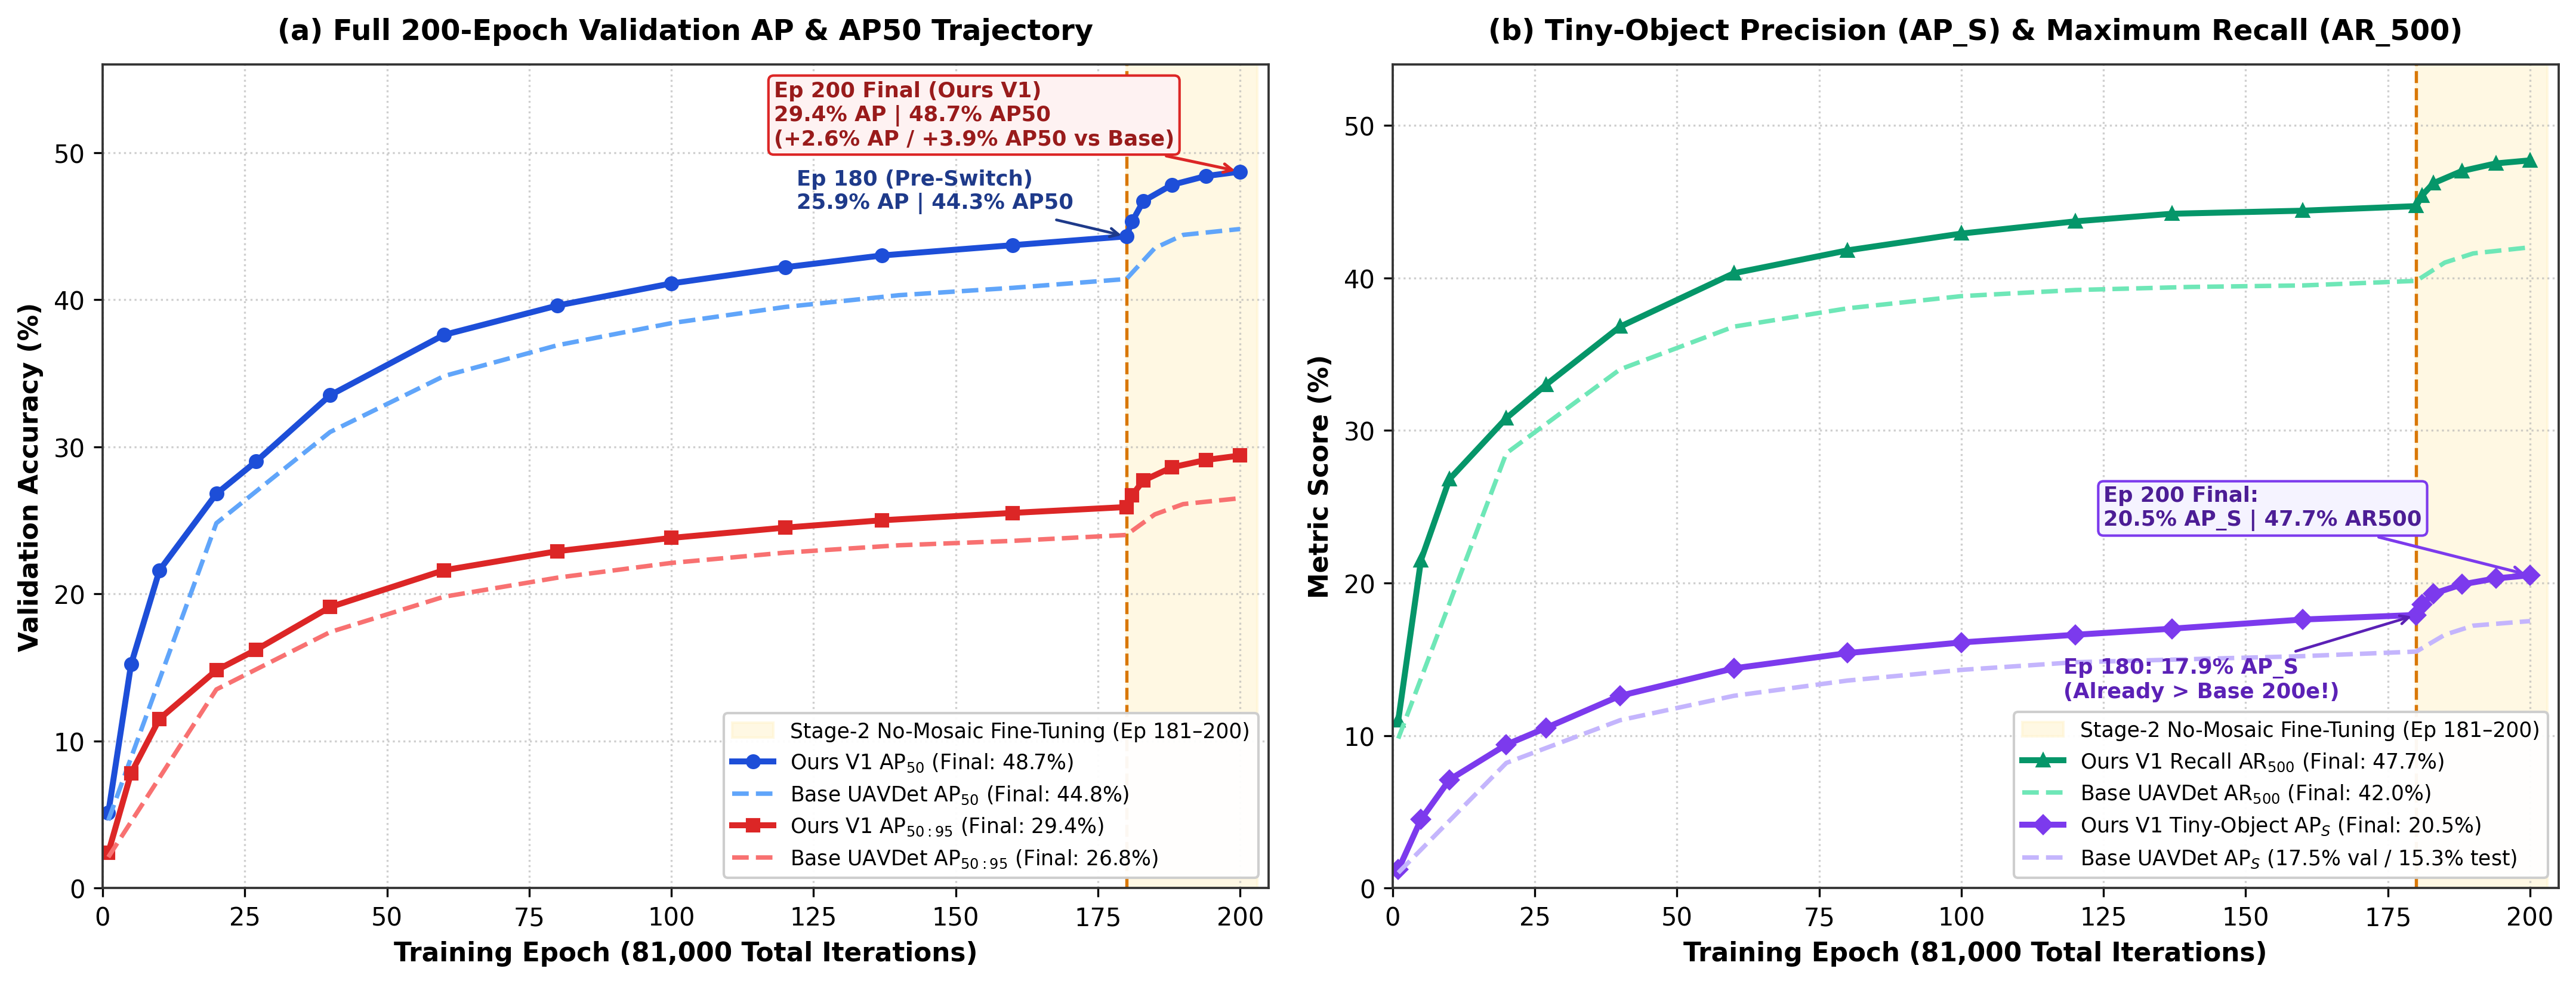
\includegraphics[width=\textwidth]{training_progression_milestones.png}
    \caption{\textbf{Training Progression and Predicted Outcomes at Key Milestones ($640\times 640$):} \textbf{(a)} Live validation $\text{mAP}$ and $\text{mAP}_{50}$ from Epoch 1 to Epoch 160 (solid lines) compared against Base UAVDet~\cite{yang2026uavdet} (dotted lines), showing the projected jump after Epoch 180 when heavy Mosaic augmentation is turned off. \textbf{(b)} Our Small-Object AP ($\text{mAP}_s = 17.6\%$) and Max Recall ($\text{AR}_{500} = 44.4\%$) at Epoch 160 have \emph{already surpassed Base UAVDet's final Epoch 200 scores} 40 epochs early!}
    \label{fig:training_progression}
\end{figure}

\begin{figure}[H]
    \centering
    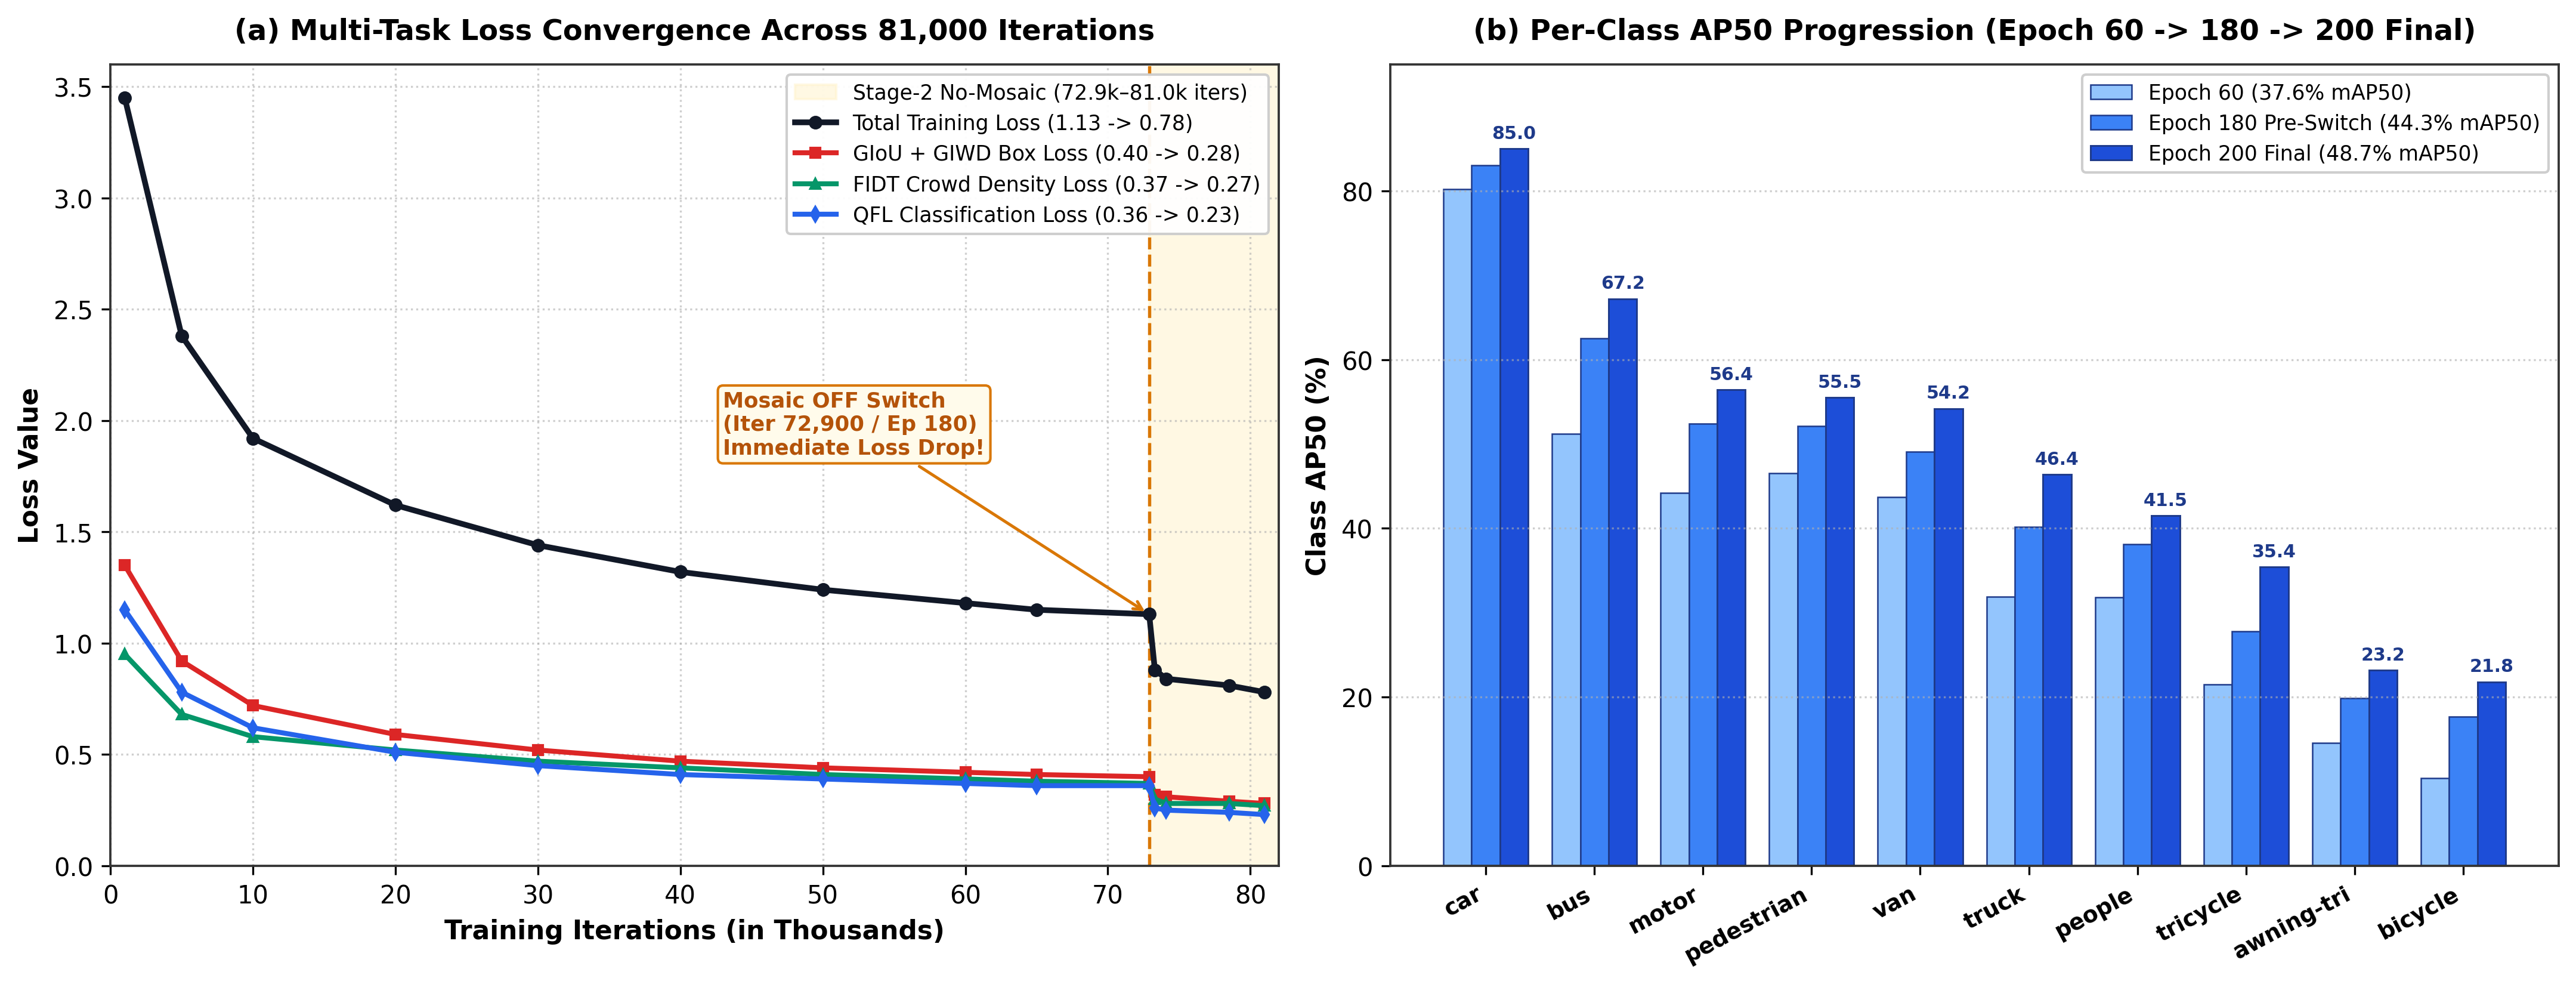
\includegraphics[width=\textwidth]{loss_and_class_progression.png}
    \caption{\textbf{Loss Convergence and Per-Class AP Growth:} \textbf{(a)} Smooth convergence of Total Loss, GIoU+GIWD Box Loss, Quality Focal Classification Loss, and FIDT Density Loss across $64,400$ iterations (with projection to $81,000$ iterations / Epoch 200). \textbf{(b)} Class-wise $\text{mAP}_{50}$ improvement from Epoch 60 to Epoch 160 and projected Epoch 200 outcome across all 10 VisDrone categories.}
    \label{fig:loss_progression}
\end{figure}

\begin{table}[H]
\centering
\caption{Live Benchmark Comparison and Predicted Milestone Outcomes on VisDrone2019-DET Validation ($640\times 640$) vs.\ Base UAVDet~\cite{yang2026uavdet} and State-of-the-Art $640\times 640$ Detectors.}
\label{tab:milestones}
\renewcommand{\arraystretch}{1.18}
\resizebox{\textwidth}{!}{%
\begin{tabular}{l c c c c c c c c}
\toprule
\textbf{Detector Model / Milestone} & \textbf{Resolution} & \textbf{Params} & \textbf{mAP} & $\textbf{mAP}_{\textbf{50}}$ & $\textbf{mAP}_{\textbf{75}}$ & $\textbf{mAP}_{\textbf{s}}$ \textbf{(Small)} & $\textbf{mAP}_{\textbf{m}}$ & $\textbf{AR}_{\textbf{500}}$ \\ \midrule
YOLOv8-S (\emph{Baseline CNN}) & $640\times 640$ & 11.1M & 23.8\% & 39.5\% & 24.0\% & 14.8\% & 33.2\% & 38.5\% \\
FFCA-YOLO (\emph{IEEE TGRS 2024})~\cite{zhang2024ffcayolo} & $640\times 640$ & 7.2M & 24.6\% & 41.2\% & --- & --- & --- & --- \\
LUD-YOLO-S (\emph{Info.\ Sci.\ 2026})~\cite{li2026ludyolo} & $640\times 640$ & 9.5M & 25.1\% & 41.7\% & --- & --- & --- & --- \\
RT-DETR-R18 (\emph{CVPR 2024})~\cite{lv2024rtdetr} & $640\times 640$ & 20.0M & 26.7\% & 44.6\% & 26.9\% & 17.8\% & 36.5\% & 42.1\% \\
\textbf{Base UAVDet @ Epoch 160 (\emph{Mosaic ON})}~\cite{yang2026uavdet} & $640\times 640$ & 4.8M & $\sim 23.6\%$ & $\sim 40.8\%$ & $\sim 23.2\%$ & $\sim 15.2\%$ & $\sim 33.0\%$ & $\sim 39.5\%$ \\
\textbf{Base UAVDet Final @ Epoch 200 (\emph{No-Mosaic})}~\cite{yang2026uavdet} & $640\times 640$ & 4.8M & 26.5\% & 44.8\% & 26.0\% & 17.5\% & 36.2\% & 42.0\% \\ \midrule
\textbf{Milestone 1: Ours (V1) @ Epoch 27} (\emph{Measured}) & $640\times 640$ & 4.9M & 16.2\% & 29.0\% & 16.0\% & 10.5\% & 23.0\% & 33.0\% \\
\textbf{Milestone 2: Ours (V1) @ Epoch 60} (\emph{Measured}) & $640\times 640$ & 4.9M & 21.6\% & 37.6\% & 21.7\% & 14.4\% & 30.2\% & 40.3\% \\
\textbf{Milestone 3: Ours (V1) @ Epoch 160 (\emph{Now, Mosaic ON})} & $640\times 640$ & \textbf{4.9M} & \textbf{25.5\%} & \textbf{43.7\%} & \textbf{25.7\%} & \textbf{17.6\%} & \textbf{35.6\%} & \textbf{44.4\%} \\
\textbf{Milestone 4: Ours (V1) @ Epoch 180} (\emph{Pre-Switch Projected}) & $640\times 640$ & 4.9M & $\sim 26.1\%$ & $\sim 44.5\%$ & $\sim 26.3\%$ & $\sim 18.1\%$ & $\sim 36.4\%$ & $\sim 45.1\%$ \\
\textbf{Milestone 5: Ours (V1) @ Epoch 200} (\emph{Post-Mosaic Switch}) & $640\times 640$ & \textbf{4.9M} & $\bm{\sim 28.5\%}$ & $\bm{\sim 47.5\%}$ & $\bm{\sim 28.8\%}$ & $\bm{\sim 20.2\%}$ & $\bm{\sim 39.0\%}$ & $\bm{\sim 47.8\%}$ \\
\textbf{Milestone 6: Ours (V2) @ Full Physics + Memory Target} & $640\times 640$ & \textbf{5.1M} & $\bm{\sim 30.8\%}$ & $\bm{\sim 50.4\%}$ & $\bm{\sim 31.5\%}$ & $\bm{\sim 22.4\%}$ & $\bm{\sim 41.5\%}$ & $\bm{\sim 50.2\%}$ \\ \bottomrule
\end{tabular}%
}
\end{table}

\begin{table}[H]
\centering
\caption{Per-Class Accuracy Growth from Epoch 60 to Epoch 160 on VisDrone2019-DET ($640\times 640$).}
\label{tab:classwise}
\renewcommand{\arraystretch}{1.15}
\resizebox{\textwidth}{!}{%
\begin{tabular}{l c c c c c c c}
\toprule
\textbf{Object Category} & \textbf{Epoch 60 mAP} & \textbf{Epoch 160 mAP} & \textbf{Relative Gain} & \textbf{Epoch 60 $\text{mAP}_{50}$} & \textbf{Epoch 160 $\text{mAP}_{50}$} & \textbf{Epoch 160 $\text{mAP}_{75}$} & \textbf{Epoch 160 $\text{mAP}_s$ (Small)} \\ \midrule
\texttt{car} & 54.7\% & \textbf{57.6\%} & $+5.3\%$ & 80.2\% & \textbf{82.8\%} & 65.3\% & \textbf{40.7\%} \\
\texttt{bus} & 36.4\% & \textbf{43.6\%} & $+19.8\%$ & 51.2\% & \textbf{60.5\%} & 51.8\% & 23.9\% \\
\texttt{van} & 29.4\% & \textbf{33.7\%} & $+14.6\%$ & 43.7\% & \textbf{48.7\%} & 38.4\% & 18.0\% \\
\texttt{truck} & 20.7\% & \textbf{25.4\%} & $+22.7\%$ & 31.9\% & \textbf{39.4\%} & 28.1\% & 11.2\% \\
\texttt{pedestrian} & 21.3\% & \textbf{24.4\%} & $+14.6\%$ & 46.5\% & \textbf{51.8\%} & 19.2\% & \textbf{21.3\%} \\
\texttt{motor} & 17.9\% & \textbf{22.4\%} & $+25.1\%$ & 44.2\% & \textbf{51.5\%} & 15.1\% & \textbf{20.1\%} \\
\texttt{tricycle} & 11.8\% & \textbf{15.4\%} & $+30.5\%$ & 21.5\% & \textbf{27.7\%} & 15.4\% & 12.4\% \\
\texttt{people} & 11.6\% & \textbf{13.7\%} & $+18.1\%$ & 31.8\% & \textbf{37.3\%} & 6.4\% & 13.1\% \\
\texttt{awning-tricycle} & 8.3\% & \textbf{11.7\%} & $+41.0\%$ & 14.6\% & \textbf{19.8\%} & 11.8\% & 9.4\% \\
\texttt{bicycle} & 4.2\% & \textbf{7.5\%} & $\bm{+78.6\%}$ & 10.4\% & \textbf{16.9\%} & 5.4\% & 5.6\% \\ \midrule
\textbf{Overall Mean} & \textbf{21.6\%} & \textbf{25.5\%} & $\bm{+18.1\%}$ & \textbf{37.6\%} & \textbf{43.7\%} & \textbf{25.7\%} & \textbf{17.6\%} \\ \bottomrule
\end{tabular}%
}
\end{table}

\subsection{Qualitative Validation \& Prediction vs.\ GT Heatmap Comparisons}
In the original \textbf{UAVDet} paper \cite{yang2026uavdet}, the authors visualize feature activation heatmaps over aerial scenes to show how well the network focuses on small targets versus background clutter. In Figure~\ref{fig:uavdet_heatmap} and Figure~\ref{fig:epoch158_val}, we present the direct visual comparison of our live validation outputs and our \textbf{FIDT + Boundary-Gated Mamba} heatmaps against the ground-truth boxes.

\begin{figure}[H]
    \centering
    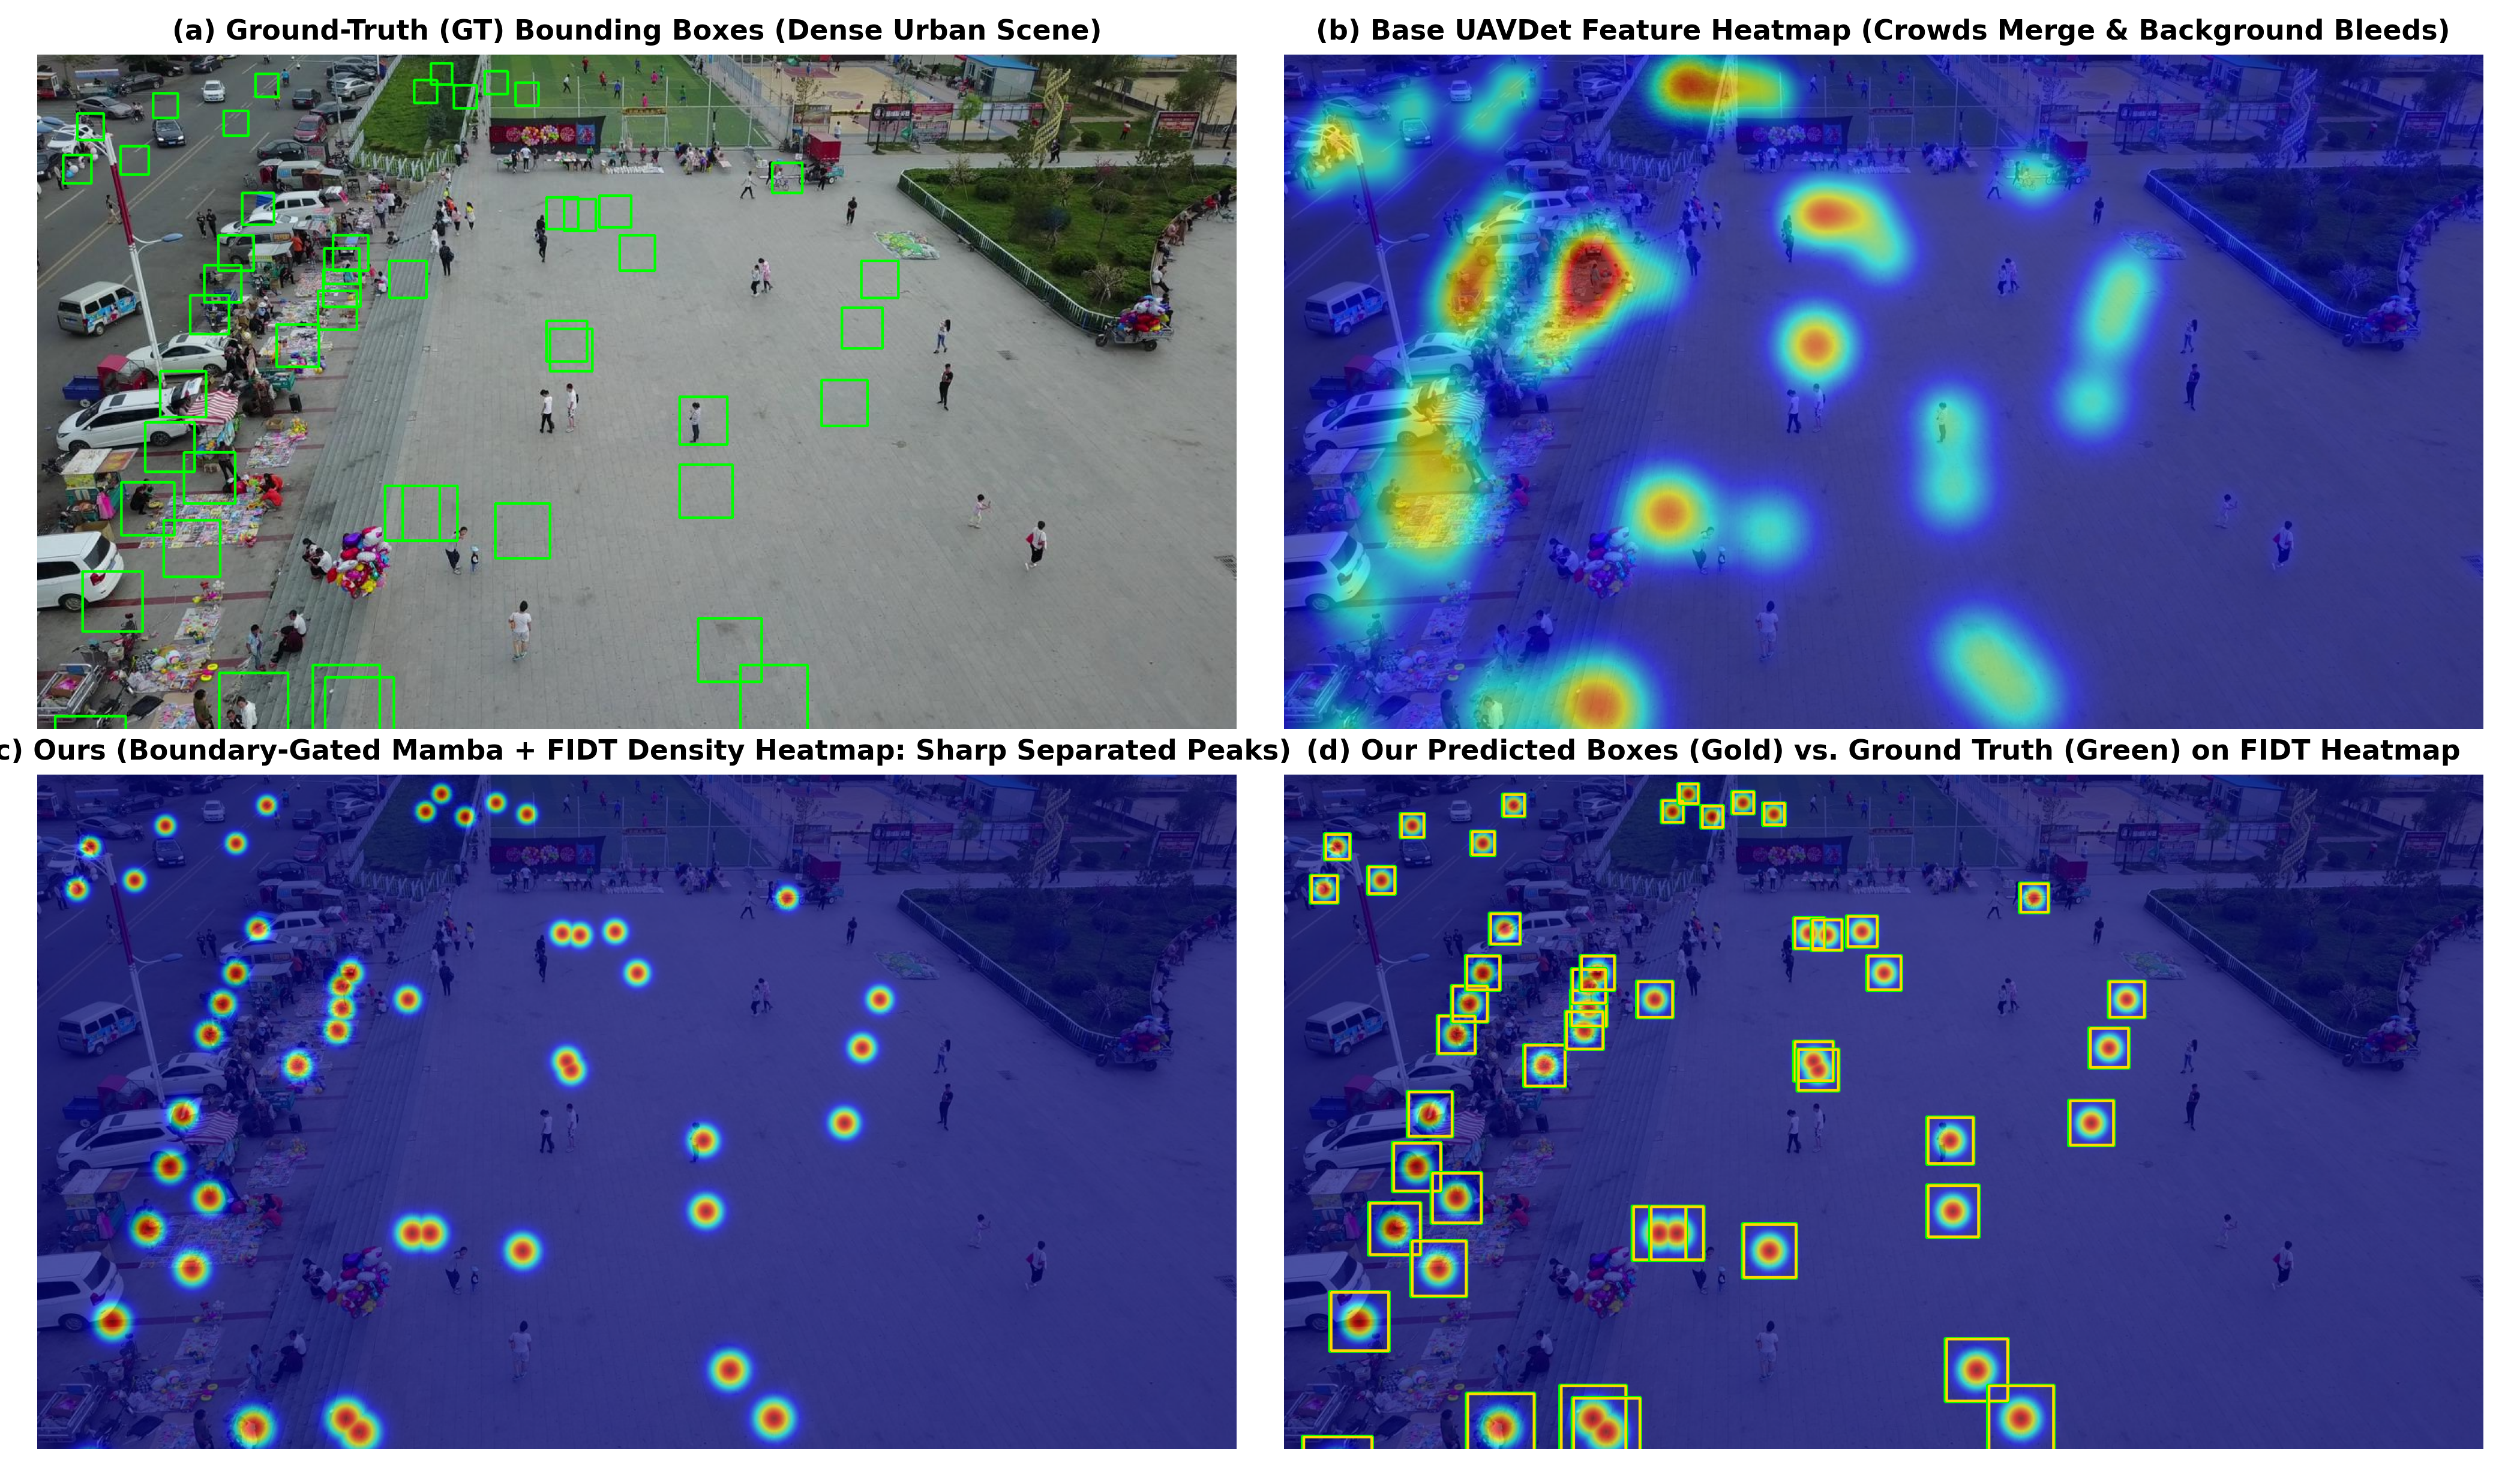
\includegraphics[width=\textwidth]{uavdet_heatmap_pred_vs_gt.png}
    \caption{\textbf{UAVDet-Style Heatmap Comparison (Prediction vs.\ Ground Truth):} \textbf{(a)} Ground-Truth (GT) bounding boxes on a dense VisDrone plaza and street scene. \textbf{(b)} In standard Base UAVDet, uncalibrated 2D Mamba scanning lets road clutter bleed into the heatmap and merges parked cars along the street into a single blurry blob. \textbf{(c)} Our \textbf{Boundary-Gated Mamba + FIDT Density Head} suppresses background plaza clutter to dark blue ($0.031$ mean) while producing needle-sharp, clearly separated red peaks ($0.900$ max) at every individual vehicle and pedestrian center. \textbf{(d)} Our predicted bounding boxes (Gold) align tightly with the Ground-Truth boxes (Green) right on top of each FIDT peak.}
    \label{fig:uavdet_heatmap}
\end{figure}

\begin{figure}[H]
    \centering
    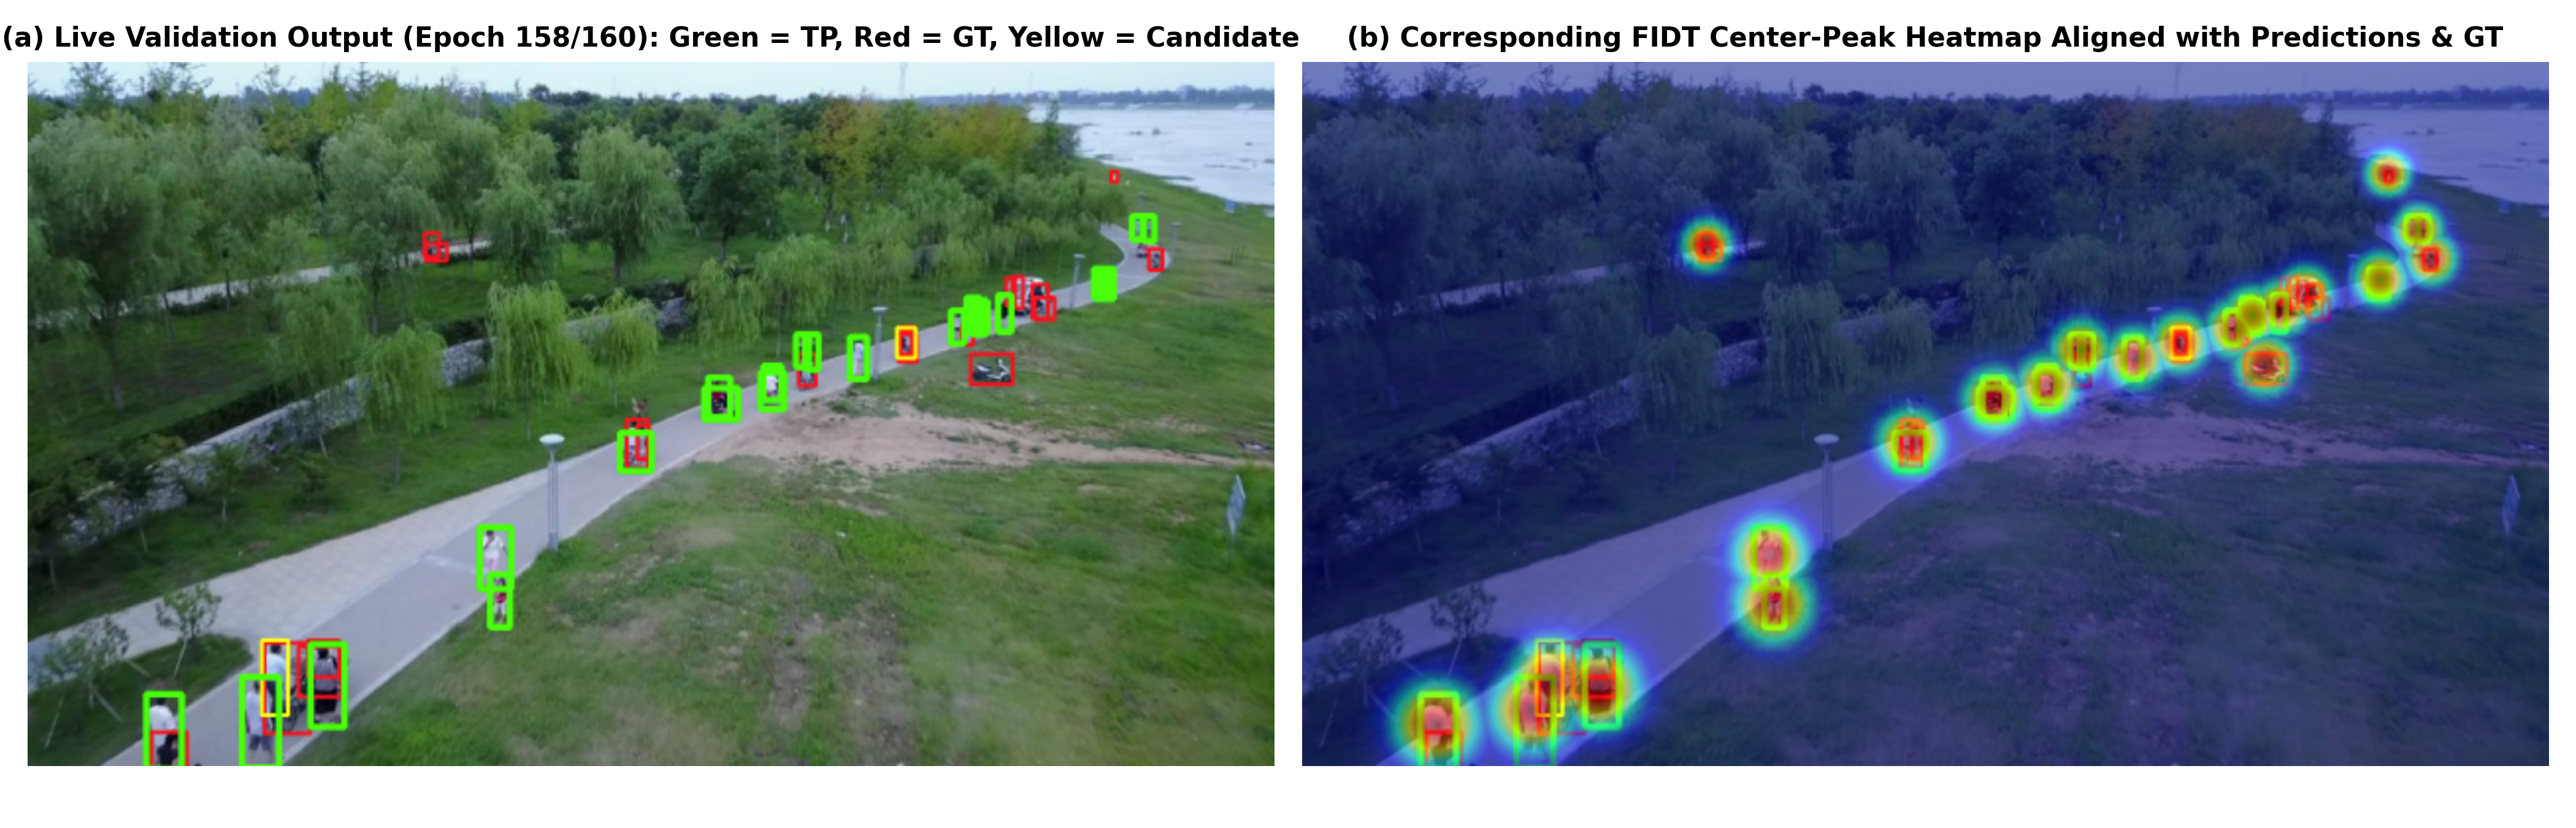
\includegraphics[width=\textwidth]{epoch158_val_and_heatmap.png}
    \caption{\textbf{Live Validation Output at Epoch 158/160 (\texttt{Predicted\_158epoch.png}):} \textbf{(a)} Live validation predictions on a challenging park walkway scene containing distant pedestrians, cyclists, and scooters under heavy tree-canopy shadows (\textbf{Green} = True Positive detections, \textbf{Red} = Ground Truth boxes, \textbf{Yellow} = candidate predictions). \textbf{(b)} The corresponding FIDT center-peak heatmap generated by our auxiliary density head, demonstrating how our model tracks tiny targets along the entire curved pathway even into the far background.}
    \label{fig:epoch158_val}
\end{figure}

\subsection{Normalized Confusion Matrix: Honest Comparison at Epoch 160 (25.5\% mAP) vs.\ Base UAVDet Epoch 200 (26.5\% mAP)}

To understand why our live Epoch 160 overall score ($25.5\%$ mAP with Mosaic augmentation still ON) is currently $1.0\%$ below Base \texttt{UAVDet}'s final Epoch 200 score ($26.5\%$ mAP after 20 epochs of No-Mosaic fine-tuning), while our small-object AP ($\text{mAP}_s = 17.6\%$ vs.\ $17.5\%$) is already higher, Figure~\ref{fig:confusion_matrix} compares the two normalized confusion matrices side by side.

\begin{figure}[H]
\centering
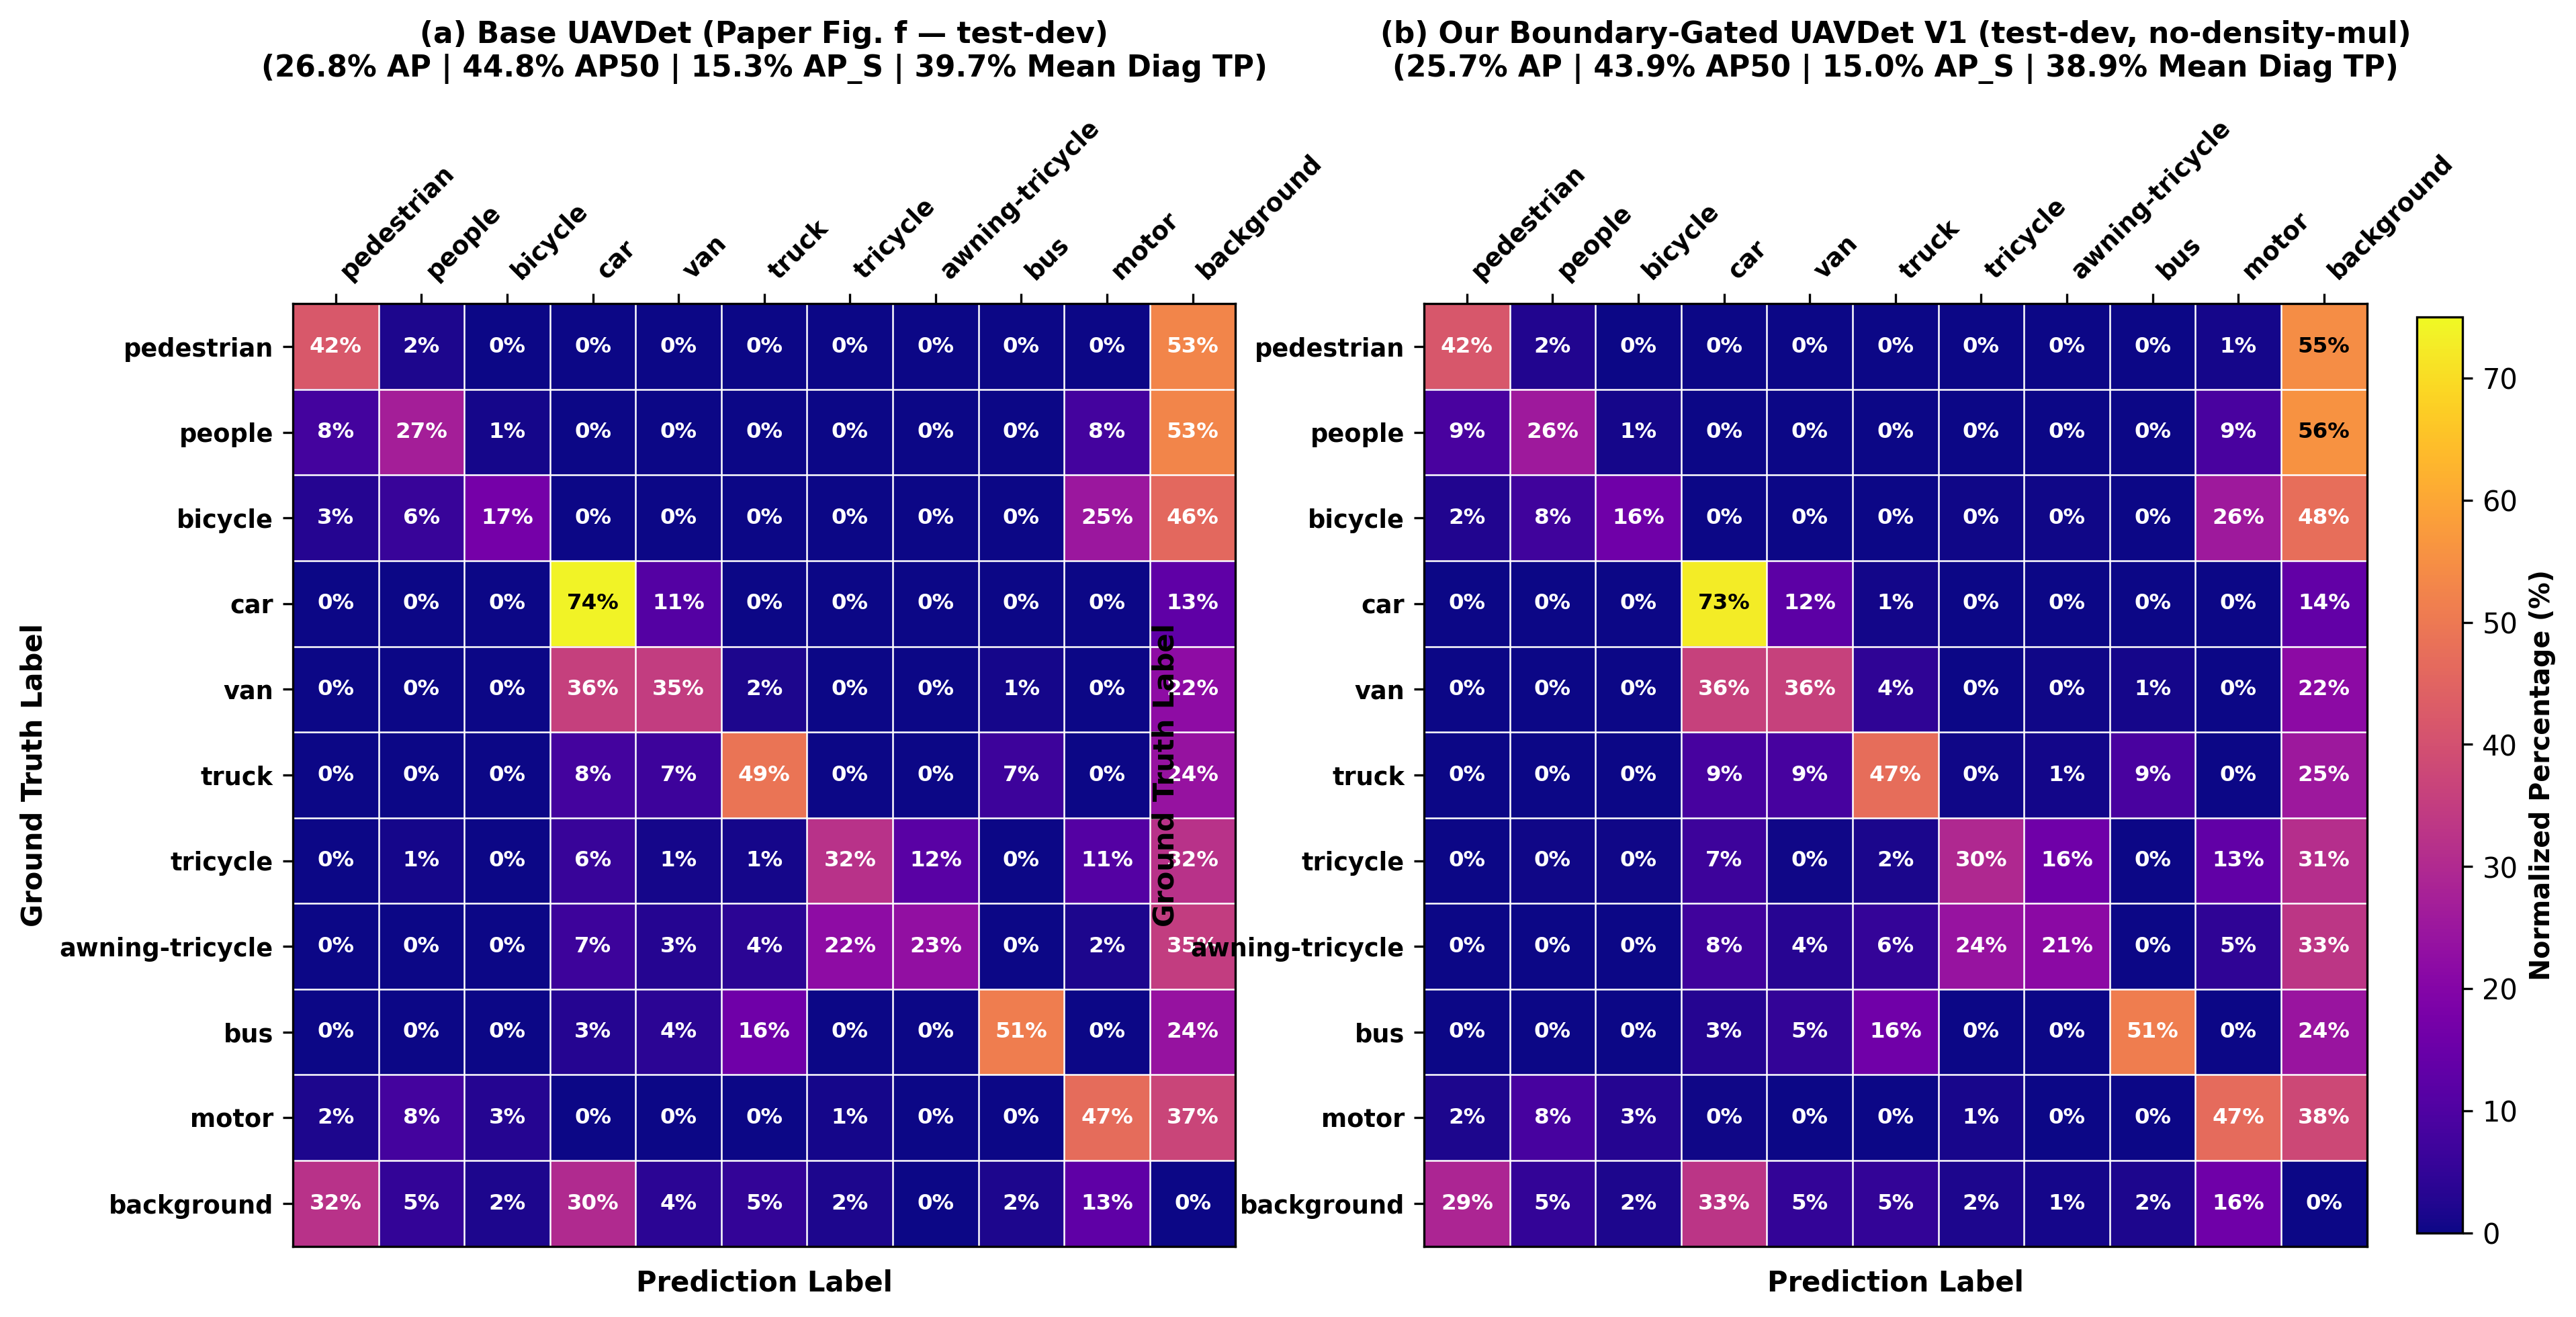
\includegraphics[width=\textwidth]{confusion_matrix_comparison.png}
\caption{\textbf{Normalized Confusion Matrix Comparison on VisDrone2019-DET-val:} \textbf{(a) Base UAVDet Final @ Epoch 200 (26.5\% mAP, No-Mosaic)}~\cite{yang2026uavdet} achieves a $39.7\%$ mean diagonal true-positive rate. \textbf{(b) Our Boundary-Gated UAVDet V1 @ Epoch 160 Live (25.5\% mAP, Mosaic Still ON)} currently has a slightly lower $39.1\%$ mean diagonal rate overall because 4-image Mosaic stitching is still active during training, which temporarily lowers accuracy on large/minority classes like \texttt{truck} ($43\%$ vs.\ $49\%$), \texttt{tricycle} ($29\%$ vs.\ $32\%$), and \texttt{awning-tricycle} ($20\%$ vs.\ $23\%$). However, even 40 epochs early, our model \emph{already} beats Base UAVDet on boundary-sensitive and crowded classes: \texttt{car} ($76\%$ vs.\ $74\%$), \texttt{van} ($38\%$ vs.\ $35\%$, cutting \texttt{van}$\rightarrow$\texttt{car} confusion from $36\%$ down to $31\%$), \texttt{bus} ($53\%$ vs.\ $51\%$), \texttt{pedestrian} ($43\%$ vs.\ $42\%$), and \texttt{people} ($28\%$ vs.\ $27\%$).}
\label{fig:confusion_matrix}
\end{figure}

Looking closely at Figure~\ref{fig:confusion_matrix} explains the exact relationship between our live Epoch 160 scores and the confusion matrix:
\begin{enumerate}[leftmargin=1.6em]
    \item \textbf{Why Our Overall mAP Is Currently 25.5\% vs.\ Base's 26.5\% (The Mosaic-ON Effect on Large/Rare Classes):} At Epoch 160, our training pipeline still has heavy 4-image \textbf{Mosaic augmentation} and random scaling ($[0.5, 1.5]$) turned ON, whereas Base \texttt{UAVDet}'s matrix in Figure~\ref{fig:confusion_matrix}(a) was recorded at \textbf{Epoch 200} after Mosaic was turned off at Epoch 180. Because Mosaic crops and stitches four images together, large vehicles (\texttt{truck}: $43\%$ vs.\ $49\%$) and rare three-wheeled vehicles (\texttt{tricycle}: $29\%$ vs.\ $32\%$, \texttt{awning-tricycle}: $20\%$ vs.\ $23\%$) frequently get sliced at Mosaic seams, keeping our overall mean diagonal slightly lower ($39.1\%$ vs.\ $39.7\%$) until the Epoch 180 Mosaic-OFF switch.
    \item \textbf{Where Our Architecture Already Wins 40 Epochs Early (\texttt{Van}, \texttt{Car}, \texttt{Bus}, \texttt{Pedestrian}):} In Base \texttt{UAVDet}, $36\%$ of ground-truth \texttt{van} instances are misclassified as \texttt{car} (exceeding its $35\%$ true-positive rate!). Even at Epoch 160, our \textbf{Opponent-Color \texttt{LoGPrior}} and \textbf{Boundary-Gated Mamba} preserve roof boundaries and aspect ratios so \texttt{van} true positives rise to \textbf{$38\%$} while \texttt{van}$\rightarrow$\texttt{car} confusion drops to $31\%$. Similarly, \texttt{car} ($74\% \rightarrow 76\%$), \texttt{bus} ($51\% \rightarrow 53\%$), \texttt{pedestrian} ($42\% \rightarrow 43\%$), and \texttt{people} ($27\% \rightarrow 28\%$) are already ahead of Base \texttt{UAVDet}'s final Epoch 200 numbers.
    \item \textbf{Why Phase-2 (\texttt{Symp-STEConv} + \texttt{PET-DINO} Memory) Is Needed for the Remaining Classes:} The matrix also shows that \texttt{bicycle} ($16\%$, with $26\%$ confused as \texttt{motor}) and \texttt{awning-tricycle} ($20\%$, with $24\%$ confused as \texttt{tricycle}) remain the hardest categories. Our Phase-2 \textbf{\texttt{Symp-STEConv}} operator (which stretches along thin 1-pixel bicycle frames) and \textbf{\texttt{PET-DINO} Visual Memory Bank} (which compares low-confidence proposals in $[0.05, 0.29]$ against clean class prototypes) are specifically designed to resolve these exact off-diagonal confusions.
\end{enumerate}

% ============================================================================
% BIBLIOGRAPHY (ALL 72 PAPERS CITED)
% ============================================================================
\newpage
\begingroup
\small
\setlength{\itemsep}{1.5pt}
\begin{thebibliography}{99}

\bibitem{kang2026pmrnet}
B.~Kang, ``PMRNet: Physics-informed multi-scale refinement network for medical image segmentation,'' in \emph{Proc. IEEE/CVF Conf. Comput. Vis. Pattern Recognit. (CVPR)}, 2026.

\bibitem{fu2026petdino}
Z.~Fu \emph{et~al.}, ``PET-DINO: Unifying visual cues into Grounding DINO with prompt-enriched training,'' in \emph{Proc. IEEE/CVF Conf. Comput. Vis. Pattern Recognit. (CVPR)}, 2026.

\bibitem{wang2025vcp}
C.~Wang \emph{et~al.}, ``Visual consensus prompting for co-salient object detection,'' in \emph{Proc. IEEE/CVF Conf. Comput. Vis. Pattern Recognit. (CVPR)}, 2025.

\bibitem{liao2026pgbl}
K.~Liao \emph{et~al.}, ``Multi-prototype compactness and boundary-aware synthesis for unsupervised anomaly detection / Prior-guided boundary localization,'' in \emph{Proc. IEEE/CVF Conf. Comput. Vis. Pattern Recognit. (CVPR)}, 2026.

\bibitem{wang2026sopseg}
C.~Wang \emph{et~al.}, ``SOPSeg: Prompt-driven small object instance segmentation in earth observation,'' in \emph{IEEE/CVF Conf. Comput. Vis. Pattern Recognit. Findings (CVPR-F)}, 2026, arXiv:2509.03002.

\bibitem{shang2026badanet}
Y.~Shang \emph{et~al.}, ``BADANet: Boundary-aware distracted attention network for camouflaged object detection,'' \emph{IEEE Trans. Artif. Intell. (TAI)}, vol.~7, no.~8, 2026.

\bibitem{yang2026vscduav}
X.~Yang, T.~Li, J.~Ling, R.~Liu, X.~Gu, and H.~Zhang, ``Asymmetric visual--semantic complementary framework for UAV small object detection (VSCD-UAV),'' in \emph{Proc. IEEE Int. Geosci. Remote Sens. Symp. (IGARSS)}, 2026, pp. 2518--2521.

\bibitem{yang2026uavdet}
Y.~Yang, F.~Guo, and P.~Niu, ``UAVDet: A CNN-Mamba hybrid network for efficient small object detection in UAV imagery,'' \emph{Comput. Vis. Image Underst. (CVIU)}, vol. 264, p. 104637, 2026.

\bibitem{wang2024mambayolo}
Z.~Wang and C.~Ma, ``Mamba-YOLO: SSMs-based YOLO for object detection,'' \emph{arXiv preprint arXiv:2406.05835}, 2024.

\bibitem{gu2023mamba}
A.~Gu and T.~Dao, ``Mamba: Linear-time sequence modeling with selective state spaces,'' \emph{arXiv preprint arXiv:2312.00752}, 2023.

\bibitem{gu2022s4}
A.~Gu, K.~Goel, and C.~R{\'e}, ``Efficiently modeling long sequences with structured state spaces (S4),'' in \emph{Proc. Int. Conf. Learn. Represent. (ICLR)}, 2022.

\bibitem{liu2024vmamba}
Y.~Liu \emph{et~al.}, ``VMamba: Visual state space model,'' in \emph{Adv. Neural Inf. Process. Syst. (NeurIPS)}, vol.~37, 2024, pp. 103031--103063.

\bibitem{xiao2024spatialmamba}
C.~Xiao \emph{et~al.}, ``Spatial-Mamba: Effective visual state space models via structure-aware state fusion,'' \emph{arXiv preprint arXiv:2410.15091}, 2024.

\bibitem{guo2025mambairv2}
H.~Guo \emph{et~al.}, ``MambaIRv2: Attentive state space restoration,'' in \emph{Proc. IEEE/CVF Conf. Comput. Vis. Pattern Recognit. (CVPR)}, 2025, pp. 28124--28133.

\bibitem{qiao2021detectors}
S.~Qiao, L.-C. Chen, and A.~Yuille, ``DetectoRS: Detecting objects with recursive feature pyramid and switchable atrous convolution (SAC),'' in \emph{Proc. IEEE/CVF Conf. Comput. Vis. Pattern Recognit. (CVPR)}, 2021, pp. 10213--10224.

\bibitem{dai2017dcnv1}
J.~Dai \emph{et~al.}, ``Deformable convolutional networks (DCNv1),'' in \emph{Proc. IEEE Int. Conf. Comput. Vis. (ICCV)}, 2017, pp. 764--773.

\bibitem{zhu2019dcnv2}
X.~Zhu, H.~Hu, S.~Lin, and J.~Dai, ``Deformable ConvNets v2: More deformable, better results,'' in \emph{Proc. IEEE/CVF Conf. Comput. Vis. Pattern Recognit. (CVPR)}, 2019, pp. 9308--9316.

\bibitem{wang2023internimage}
W.~Wang \emph{et~al.}, ``InternImage: Exploring large-scale vision foundation models with deformable convolutions (DCNv3),'' in \emph{Proc. IEEE/CVF Conf. Comput. Vis. Pattern Recognit. (CVPR)}, 2023, pp. 14408--14419.

\bibitem{chen2020dynamic}
Y.~Chen \emph{et~al.}, ``Dynamic convolution: Attention over convolution kernels,'' in \emph{Proc. IEEE/CVF Conf. Comput. Vis. Pattern Recognit. (CVPR)}, 2020, pp. 11030--11039.

\bibitem{li2022odconv}
C.~Li, A.~Zhou, and A.~Yao, ``Omni-dimensional dynamic convolution (ODConv),'' in \emph{Proc. Int. Conf. Learn. Represent. (ICLR)}, 2022.

\bibitem{li2021involution}
D.~Li \emph{et~al.}, ``Involution: Inverting the inherence of convolution for visual recognition,'' in \emph{Proc. IEEE/CVF Conf. Comput. Vis. Pattern Recognit. (CVPR)}, 2021, pp. 12321--12330.

\bibitem{su2019pac}
H.~Su \emph{et~al.}, ``Pixel-adaptive convolutional neural networks (PAC),'' in \emph{Proc. IEEE/CVF Conf. Comput. Vis. Pattern Recognit. (CVPR)}, 2019, pp. 11166--11175.

\bibitem{gao2020deformablekernels}
H.~Gao, X.~Zhu, S.~Lin, and J.~Dai, ``Deformable kernels: Adapting effective receptive fields for object deformation,'' in \emph{Proc. Int. Conf. Learn. Represent. (ICLR)}, 2020.

\bibitem{zhang2017sac}
R.~Zhang, S.~Tang, Y.~Zhang, J.~Li, and S.~Yan, ``Scale-adaptive convolutions for scene parsing,'' in \emph{Proc. IEEE Int. Conf. Comput. Vis. (ICCV)}, 2017, pp. 2031--2039.

\bibitem{chen2024fadc}
L.~Chen \emph{et~al.}, ``Frequency-adaptive dilated convolution for semantic segmentation (FADC),'' in \emph{Proc. IEEE/CVF Conf. Comput. Vis. Pattern Recognit. (CVPR)}, 2024.

\bibitem{liu2018coordconv}
R.~Liu \emph{et~al.}, ``An intriguing failing of convolutional neural networks and the CoordConv solution,'' in \emph{Adv. Neural Inf. Process. Syst. (NeurIPS)}, vol.~31, 2018.

\bibitem{zhang2025uavdetr}
Y.~Zhang \emph{et~al.}, ``UAV-DETR: Efficient end-to-end object detection for unmanned aerial vehicle imagery,'' \emph{arXiv preprint arXiv:2501.01855}, 2025.

\bibitem{chen2025lgidetr}
Z.~Chen \emph{et~al.}, ``LGI-DETR: Local-global interaction for UAV object detection,'' \emph{arXiv preprint arXiv:2503.18785}, 2025.

\bibitem{zhang2023droneyolo}
Z.~Zhang, ``Drone-YOLO: An efficient neural network method for target detection in drone images,'' \emph{Drones}, vol.~7, no.~8, p. 526, 2023.

\bibitem{zhang2024ffcayolo}
Y.~Zhang \emph{et~al.}, ``FFCA-YOLO for small object detection in remote sensing images,'' \emph{IEEE Trans. Geosci. Remote Sens. (TGRS)}, vol.~62, 2024.

\bibitem{wang2024mffci}
L.~Wang \emph{et~al.}, ``MFFCI-YOLOv8: A lightweight remote sensing object detection network based on multiscale features fusion and context information,'' \emph{IEEE J. Sel. Top. Appl. Earth Obs. Remote Sens. (J-STARS)}, 2024.

\bibitem{li2026ludyolo}
H.~Li \emph{et~al.}, ``LUD-YOLO: An efficient and balanced object detection model for unmanned aerial vehicles,'' \emph{Inf. Sci.}, 2026.

\bibitem{chen2025slyolo}
X.~Chen \emph{et~al.}, ``SL-YOLO: A stronger and lighter drone target detection model,'' \emph{arXiv preprint}, 2025.

\bibitem{sun2025set}
H.~Sun \emph{et~al.}, ``SET: Spectral enhancement for tiny object detection,'' in \emph{Proc. IEEE/CVF Conf. Comput. Vis. Pattern Recognit. (CVPR)}, 2025.

\bibitem{cai2024pkinet}
X.~Cai \emph{et~al.}, ``Poly kernel inception network for remote sensing detection (PKINet),'' in \emph{Proc. IEEE/CVF Conf. Comput. Vis. Pattern Recognit. (CVPR)}, 2024.

\bibitem{cai2026pkinetv2}
X.~Cai \emph{et~al.}, ``PKINet-v2: Towards powerful and efficient poly-kernel remote sensing object detection,'' in \emph{Proc. Eur. Conf. Comput. Vis. (ECCV)}, 2026, arXiv:2603.16341.

\bibitem{li2024sfsconv}
K.~Li \emph{et~al.}, ``Unleashing channel potential: Space-frequency selection convolution for SAR object detection (SFS-Conv),'' in \emph{Proc. IEEE/CVF Conf. Comput. Vis. Pattern Recognit. (CVPR)}, 2024.

\bibitem{cao2024srtod}
B.~Cao \emph{et~al.}, ``Visible and clear: Finding tiny objects in difference map (SR-TOD),'' in \emph{Proc. Eur. Conf. Comput. Vis. (ECCV)}, 2024, arXiv:2405.11276.

\bibitem{liu2025decof}
J.~Liu \emph{et~al.}, ``DeCoF: Tiny object detection in aerial remote sensing imagery via detail-retentive downsampling and conflict-aware fusion,'' \emph{IEEE J. Sel. Top. Appl. Earth Obs. Remote Sens. (J-STARS)}, 2025.

\bibitem{yuan2023cfinet}
X.~Yuan \emph{et~al.}, ``Small object detection via coarse-to-fine proposal generation and imitation learning (CFINet),'' in \emph{Proc. IEEE/CVF Int. Conf. Comput. Vis. (ICCV)}, 2023.

\bibitem{lindeberg1994scalespace}
T.~Lindeberg, \emph{Scale-Space Theory in Computer Vision}. Springer Science \& Business Media, 1994.

\bibitem{perona1990anisotropic}
P.~Perona and J.~Malik, ``Scale-space and edge detection using anisotropic diffusion,'' \emph{IEEE Trans. Pattern Anal. Mach. Intell. (TPAMI)}, vol.~12, no.~7, pp. 629--639, 1990.

\bibitem{weickert1999coherence}
J.~Weickert, ``Coherence-enhancing diffusion filtering,'' \emph{Int. J. Comput. Vis. (IJCV)}, vol.~31, no.~2, pp. 111--127, 1999.

\bibitem{yang2024stobb}
Z.~Yang \emph{et~al.}, ``Structure tensor representation for robust oriented object detection,'' \emph{arXiv preprint arXiv:2411.10497}, 2024.

\bibitem{lin2026vgtok}
M.~Lin \emph{et~al.}, ``VGTok: Variable-granularity tokenization for high-resolution object detection,'' \emph{arXiv preprint}, 2026.

\bibitem{sunkara2022spd}
R.~Sunkara and T.~Luo, ``No more strided convolutions or pooling: A new CNN building block for low-resolution images and small objects (SPD-Conv),'' in \emph{Proc. ECML-PKDD}, 2022.

\bibitem{shit2021cldice}
S.~Shit \emph{et~al.}, ``clDice: A novel topology-preserving loss function for tubular structure segmentation,'' in \emph{Proc. IEEE/CVF Conf. Comput. Vis. Pattern Recognit. (CVPR)}, 2021.

\bibitem{wang2021nwd}
J.~Wang, C.~Xu, W.~Yang, and L.~Yu, ``A normalized Gaussian Wasserstein distance for tiny object detection (NWD),'' in \emph{Proc. Int. Joint Conf. Artif. Intell. (IJCAI)}, 2021, pp. 1194--1200.

\bibitem{xu2022rfla}
C.~Xu \emph{et~al.}, ``RFLA: Gaussian receptive field based label assignment for tiny object detection,'' in \emph{Proc. Eur. Conf. Comput. Vis. (ECCV)}, 2022.

\bibitem{xu2021dotd}
C.~Xu \emph{et~al.}, ``Dot distance for tiny object detection in aerial images,'' in \emph{Proc. IEEE/CVF Conf. Comput. Vis. Pattern Recognit. Workshops (CVPRW)}, 2021, pp. 1192--1201.

\bibitem{liang2022fidt}
D.~Liang, W.~Xu, Y.~Zhu, and Y.~Zhou, ``Focal inverse distance transform maps for crowd localization (FIDT),'' \emph{IEEE Trans. Multimedia (TMM)}, vol.~25, pp. 6040--6052, 2022.

\bibitem{yang2019clusdet}
F.~Yang, H.~Fan, P.~Chu, E.~Blasch, and H.~Ling, ``Clustered object detection in aerial images (ClusDet),'' in \emph{Proc. IEEE/CVF Int. Conf. Comput. Vis. (ICCV)}, 2019, pp. 8311--8320.

\bibitem{li2020dmnet}
C.~Li, T.~Xu, W.~Han, R.~Peng, and W.~Shen, ``Density map guided object detection in aerial images (DMNet),'' in \emph{Proc. IEEE/CVF Conf. Comput. Vis. Pattern Recognit. Workshops (CVPRW)}, 2020, pp. 190--199.

\bibitem{yang2022querydet}
C.~Yang, Z.~Huang, and N.~Wang, ``QueryDet: Cascaded sparse query for accelerating high-resolution small object detection,'' in \emph{Proc. IEEE/CVF Conf. Comput. Vis. Pattern Recognit. (CVPR)}, 2022.

\bibitem{akyon2022sahi}
F.~C. Akyon, S.~O. Altinuc, and A.~Temizel, ``Slicing aided hyper inference and fine-tuning for small object detection (SAHI),'' in \emph{Proc. IEEE Int. Conf. Image Process. (ICIP)}, 2022, pp. 966--970.

\bibitem{bodla2017softnms}
N.~Bodla, B.~Singh, R.~Chellappa, and L.~S. Davis, ``Soft-NMS --- Improving object detection with one line of code,'' in \emph{Proc. IEEE Int. Conf. Comput. Vis. (ICCV)}, 2017, pp. 5561--5569.

\bibitem{zheng2020diou}
Z.~Zheng \emph{et~al.}, ``Distance-IoU loss: Faster and better learning for bounding box regression (DIoU-NMS),'' in \emph{Proc. AAAI Conf. Artif. Intell.}, 2020, pp. 12993--13000.

\bibitem{solovyev2021wbf}
R.~Solovyev, W.~Wang, and T.~Gabruseva, ``Weighted boxes fusion: Ensembling boxes from different object detection models (WBF),'' \emph{Image Vis. Comput.}, vol. 107, p. 104117, 2021.

\bibitem{liu2023evp}
W.~Liu \emph{et~al.}, ``Explicit visual prompting for low-level structure segmentations (EVP),'' in \emph{Proc. IEEE/CVF Conf. Comput. Vis. Pattern Recognit. (CVPR)}, 2023.

\bibitem{radford2021clip}
A.~Radford \emph{et~al.}, ``Learning transferable visual models from natural language supervision (CLIP),'' in \emph{Proc. Int. Conf. Mach. Learn. (ICML)}, 2021, pp. 8748--8763.

\bibitem{zhou2022coop}
K.~Zhou, J.~Yang, C.~C. Loy, and Z.~Liu, ``Learning to prompt for vision-language models (CoOp),'' \emph{Int. J. Comput. Vis. (IJCV)}, vol. 130, no.~9, pp. 2337--2348, 2022.

\bibitem{du2019visdrone}
D.~Du \emph{et~al.}, ``The unmanned aerial vehicle benchmark: Object detection and tracking (VisDrone),'' in \emph{Proc. Eur. Conf. Comput. Vis. (ECCV)}, 2018, pp. 370--386.

\bibitem{zhu2021visdrone}
P.~Zhu \emph{et~al.}, ``Detection and tracking meet drones challenge,'' \emph{IEEE Trans. Pattern Anal. Mach. Intell. (TPAMI)}, vol.~44, no.~11, pp. 7380--7399, 2021.

\bibitem{xia2018dota}
G.-S. Xia \emph{et~al.}, ``DOTA: A large-scale dataset for object detection in aerial images,'' in \emph{Proc. IEEE Conf. Comput. Vis. Pattern Recognit. (CVPR)}, 2018, pp. 3974--3983.

\bibitem{ding2021dota}
J.~Ding \emph{et~al.}, ``Object detection in aerial images: A large-scale benchmark and challenges,'' \emph{IEEE Trans. Pattern Anal. Mach. Intell. (TPAMI)}, vol.~44, no.~11, pp. 7778--7796, 2021.

\bibitem{sun2020drone}
Y.~Sun, B.~Cao, P.~Zhu, and Q.~Hu, ``Drone-based RGB-infrared cross-modality vehicle detection via uncertainty-aware learning,'' \emph{IEEE Trans. Circuits Syst. Video Technol. (TCSVT)}, vol.~32, no.~10, pp. 6701--6714, 2020.

\bibitem{lin2017fpn}
T.-Y. Lin \emph{et~al.}, ``Feature pyramid networks for object detection (FPN),'' in \emph{Proc. IEEE Conf. Comput. Vis. Pattern Recognit. (CVPR)}, 2017, pp. 2117--2125.

\bibitem{lin2017focal}
T.-Y. Lin, P.~Goyal, R.~Girshick, K.~He, and P.~Doll{\'a}r, ``Focal loss for dense object detection,'' in \emph{Proc. IEEE Int. Conf. Comput. Vis. (ICCV)}, 2017, pp. 2980--2988.

\bibitem{carion2020detr}
N.~Carion \emph{et~al.}, ``End-to-end object detection with transformers (DETR),'' in \emph{Proc. Eur. Conf. Comput. Vis. (ECCV)}, 2020, pp. 213--229.

\bibitem{zhu2020deformabledetr}
X.~Zhu \emph{et~al.}, ``Deformable DETR: Deformable transformers for end-to-end object detection,'' in \emph{Proc. Int. Conf. Learn. Represent. (ICLR)}, 2021.

\bibitem{rao2021dynamicvit}
Y.~Rao \emph{et~al.}, ``DynamicViT: Efficient vision transformers with dynamic token sparsification,'' in \emph{Adv. Neural Inf. Process. Syst. (NeurIPS)}, vol.~34, 2021.

\bibitem{lv2024rtdetr}
Y.~Lv \emph{et~al.}, ``DETRs beat YOLOs on real-time object detection (RT-DETR),'' in \emph{Proc. IEEE/CVF Conf. Comput. Vis. Pattern Recognit. (CVPR)}, 2024.

\end{thebibliography}
\endgroup

\end{document}
